\documentclass[a4paper,12pt,twoside]{report}
%%%%%%%%%%%%%%%%%%%%%%%%%%%%
% University of Sussex thesis template
%%%%%%%%%%%%%%%%%%%%%%%%%%%%


%%%%%%%%%%%%%%%%%%%%%%%%%%%%
% LINE SPACING
\newcommand{\linespacing}{1.5}
\renewcommand{\baselinestretch}{\linespacing}
%%%%%%%%%%%%%%%%%%%%%%%%%%%%


%%%%%%%%%%%%%%%%%%%%%%%%%%%%
% BIBLIOGRAPHY STYLE
\usepackage{plain}
\bibliographystyle{utphys}
%%%%%%%%%%%%%%%%%%%%%%%%%%%%


%%%%%%%%%%%%%%%%%%%%%%%%%%%%
% OTHER FORMATTING/LAYOUT DECLARATIONS
% Graphics
\usepackage{graphicx,color}
\usepackage{epstopdf}
\usepackage[british]{babel}
\graphicspath{{Images/}}
% The left-hand-side should be 40mm.  The top and bottom margins should be
% 25mm deep.  The right hand margin should be 20mm.
\usepackage[a4paper,top=2.5cm,bottom=2.5cm,left=3cm,right=2cm,headsep=10pt]{geometry}
\flushbottom
% Pages should be numbered consecutively thorugh the main text.  Page numbers
% should be located centrally at the top of the page.
\usepackage{fancyhdr}
\fancypagestyle{plain}{
	\fancyhf{}
	% Add "DRAFT: <today's date>" to header (comment out the following to remove)
	\fancyhead[LE,RO]{\textit{MPhys Final Year Project - Scalar Fields in Cosmology}}
	%
	\fancyfoot[LE,RO]{\thepage}
	\renewcommand{\headrulewidth}{0pt}
}
\pagestyle{plain}
%%%%%%%%%%%%%%%%%%%%%%%%%%%%


%%%%%%%%%%%%%%%%%%%%%%%%%%%%
% ANY OTHER DECLARATIONS HERE:

%%%%%%%%%%%%%%%%%%%%%%%%%%%%


%%%%%%%%%%%%%%%%%%%%%%%%%%%%
% HYPERREF
%\usepackage[colorlinks,pagebackref,pdfusetitle,urlcolor=blue,citecolor=blue,linkcolor=blue,bookmarksnumbered,plainpages=false]{hyperref}
\usepackage{amsmath}
\usepackage{amssymb}
\newcommand{\abs}[1]{\lvert#1\rvert}
\usepackage{tikz}
\usepackage{caption}
\usepackage{xfrac}
\usepackage{tensor}
\usepackage{braket}

% For print version, use this instead:
%\usepackage[pdfusetitle,bookmarksnumbered,plainpages=false,backref=page]{hyperref}
%\usepackage[hyperpageref]{backref}
%\renewcommand{\backrefpagesname}{Cited on}
%%%%%%%%%%%%%%%%%%%%%%%%%%%%

\usepackage[pdftex,pagebackref]{hyperref}
    \usepackage{plain}
    \hypersetup{colorlinks,urlcolor=blue,citecolor=blue,linkcolor=blue,linktocpage=true}
\renewcommand{\backrefpagesname}{ \protect  \textit{Cited on
page(s):}~}
\renewcommand{\backref}{\backrefpagesname}

%%%%%%%%%%%%%%%%%%%%%%%%%%%%
% Rectangled Numbers
\newcommand*\myrect[1]{%
  \begin{tikzpicture}[baseline=(R.base)]
    \node[draw,rectangle,inner sep=2.0pt](R) {#1};
  \end{tikzpicture}}
% Circled Numbers
\newcommand*\circled[1]{\tikz[baseline=(char.base)]{
            \node[shape=circle,draw,inner sep=2pt] (char) {#1};}}
%%%%%%%%%%%%%%%%%%%%%%%%%%%%

% Code formatting package
\usepackage{listings}
\usepackage{color}

\definecolor{dkgreen}{rgb}{0,0.6,0}
\definecolor{gray}{rgb}{0.5,0.5,0.5}
\definecolor{mauve}{rgb}{0.58,0,0.82}

\lstset{frame=tb,
  language=Python,
  aboveskip=3mm,
  belowskip=3mm,
  showstringspaces=false,
  columns=flexible,
  basicstyle={\small\ttfamily},
  numbers=none,
  numberstyle=\tiny\color{gray},
  keywordstyle=\color{blue},
  commentstyle=\color{dkgreen},
  stringstyle=\color{mauve},
  breaklines=true,
  breakatwhitespace=true
  tabsize=3
}
%%%%%%%%%%%%%%%%%%%%%%%%%%%%

%%%%%%%%%%%%%%%%%%%%%%%%%%%%
% BEGIN DOCUMENT
\begin{document}
%%%%%%%%%%%%%%%%%%%%%%%%%%%%


%%%%%%%%%%%%%%%%%%%%%%%%%%%%
% PREAMBLE: roman page numbering i, ii, iii, ...
\pagenumbering{arabic}
%%%%%%%%%%%%%%%%%%%%%%%%%%%%


%%%%%%%%%%%%%%%%%%%%%%%%%%%%
%% TITLE PAGE: The title page should give the following information:
%%	(i) the full title of the thesis and the sub-title if any;
%%	(ii) the full name of the author;
%%	(iii) the qualification aimed for;
%%	(iv) the name of the University of Sussex;
%%	(v) the month and year of submission.
\thispagestyle{empty}
\begin{flushright}
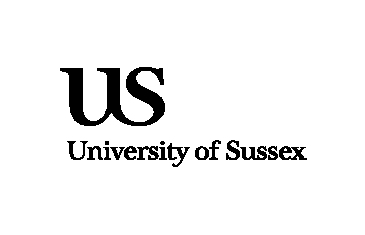
\includegraphics[width=6cm]{uslogo}
\end{flushright}	
\vskip40mm
\begin{center}
% TITLE
\huge\textbf{Scalar Fields in Cosmology}
\vskip2mm
% SUBTITLE (optional)
\LARGE\textit{MPhys Final Year Project}
\vskip5mm
% AUTHOR
\Large\textbf{Candidate Number: 78639}
\vskip5mm
\Large\textit{Supervisor: Prof Mark Hindmarsh, Professor in Theoretical Physics}
\normalsize
\end{center}
\vfill
\begin{flushleft}
\large
% QUALIFICATION
Physics \& Astronomy \\
University of Sussex	\\
% DATE OF SUBMISSION
May 7 2015
\end{flushleft}		
%%%%%%%%%%%%%%%%%%%%%%%%%%%%


%%%%%%%%%%%%%%%%%%%%%%%%%%%%
% SUMMARY PAGE
\thispagestyle{empty}
\newpage
\null\vskip10mm
\begin{center}
\large
\underline{UNIVERSITY OF SUSSEX}
\vskip15mm
% AUTHOR, QUALIFICATION
\textsc{Candidate Number: 78639}
\vskip15mm
% TITLE
\underline{\textsc{Scalar Fields in Cosmology}}
\vskip15mm
% SUBTITLE (optional)
\underline{\textsc{Abstract}}
\vskip15mm
\end{center}
% Change line spacing
\renewcommand{\baselinestretch}{1.0}
\small\normalsize
% SUMMARY HERE (300 word limit for most subjects):

\noindent Here we discuss the principles of modern cosmology before describing the three major problems with it and explore how inflation generated by a scalar field can solve these problems. By defining some conditions required to solve these problems, we show that the equation of motion for this scalar field in a curved spacetime fulfils the conditions and hence solves the problems. The Friedmann equations are then written in terms of the scalar field and its potential which shows that the field must be changing very slowly compared with the potential under the slow-roll approximation with corresponding parameters. By introducing inhomogeneities in the scalar field and the spacetime metric, we then show that when quantised, they obey another equation of motion whose solutions give observables in the cosmic microwave background related to the origin of large-scale structure. These equations of motion are solved numerically without using the slow-roll approximation or any assumption about spacetime and the results compared with the most recent Planck results.

%%%%%%%%%%%%%%%%%%%%%%%%%%%%


%%%%%%%%%%%%%%%%%%%%%%%%%%%%
% TABLE OF CONTENTS, LISTS OF TABLES & FIGURES
\newpage
\pdfbookmark[0]{Contents}{contents_bookmark}
\tableofcontents
%\listoftables
%\phantomsection
%\addcontentsline{toc}{chapter}{List of Tables}
\listoffigures
\phantomsection
\addcontentsline{toc}{chapter}{List of Figures}
%%%%%%%%%%%%%%%%%%%%%%%%%%%%


%%%%%%%%%%%%%%%%%%%%%%%%%%%%
% MAIN THESIS TEXT: arabic page numbering 1, 2, 3, ...
\newpage
%\pagenumbering{arabic}
%%%%%%%%%%%%%%%%%%%%%%%%%%%%


%-----------------------------------------------------
% Chapter: Introduction
%-----------------------------------------------------

% NB Good idea to put each chapter in a separate file.
% If you put the following in a file called "thesis_introduction.tex"
% then you can include it with the following:

% \input{thesis_introduction}

\chapter{Introduction}
\label{chap:intro}

\section{Preface} \label{sec:Preface}

In this paper, we will discuss building a program that solves differential equations for the evolution of a scalar field in the early universe and computes power spectra from the solution. Initially, a paper by Ringeval \cite{Ringeval:2007am} was used to develop an understanding of the physical requirements that needed to be satisfied in the code. Once I had written the first version of the program, I was given assistance with debugging and testing by my supervisor Prof Mark Hindmarsh.

\section{A History of Inflationary Cosmology} \label{sec:HistInflatCosmo}

At the turn of the 20th century, the study of cosmology went through a grand transition when Einstein first published his general theory of relativity \cite{Einstein:1916vd}. Since then, the study has continued at a great pace and at present we are undergoing the next major revolution in our understanding with high-precision cosmology. The inflationary paradigm was first proposed by Alan Guth in 1981 \cite{Guth:1980zm} and describes an accelerating expansion during the early universe that provides an elegant solution to many of the problems in cosmology prior at the time. After that, Andrei Linde expanded on this by proposing slow-roll inflation where the expansion is generated by a scalar field rolling slowly down a potential \cite{Linde:1981mu}. Viatcheslav Mukhanov then showed how quantum fluctuations in the scalar field are generated that were the precursors to all of the structure seen in the universe today \cite{Mukhanov:1981xt}. Today we find ourselves able to observe the signatures left by these early fluctuations using telescopes such as Planck and test the inflation framework in detail.

\section{Layout of Report} \label{sec:LayReport}

In the background theory chapter, we shall begin a discussion of the problems with the current big bang model and then develop the inflationary paradigm as a means of solving these problems. This will begin by establishing the conditions needed for inflation and then showing that they are satisfied by deriving an equation of motion for a scalar field in curved spacetime. Next we will develop a theory for inhomogeneities in the scalar field and compute power spectra that describes these using quantum field theory. We will then have a numerical methods chapter that describes how we implement these theories using a Python code including any transformations or equations needed. The results of this program will then be presented for three separate potentials before discussing their validity in the context of recent studies. Throughout this report, we will assume natural units where $\hbar = c = 1$ and use roman indices (i, j,..) for spatial components with greek indices ($\mu, \nu,...$) used for spacetime components. Any other conventions will be mentioned in the text.


%-----------------------------------------------------
% Chapter: Background Theory
%-----------------------------------------------------

\chapter{Background Theory}
\label{chap:BgTheory}

Today, physicists use the Lambda Cold Dark Matter ($\Lambda$CDM) model of cosmology, which allows the big bang model to be defined as a set of parameters that determine the properties of the universe on a large scale. Some of these parameters include the proportion of baryon content and the age of the universe. However, the $\Lambda$CDM model does have particular problems that leave some observed physical properties unexplained which is where inflation driven by scalar fields helps resolve these issues. In this chapter, we will first discuss the Friedmann equations before identifying and quantifying the fore-mentioned problems in the model. Next, we shall introduce the inflationary paradigm before demonstrating how the $\Lambda$CDM model's problems are fixed by the postulates introduced by inflation. We will then introduce scalar field theory to show how it can produce some of the properties required from inflation and derive an equation of motion in a curved spacetime. Finally, the theory of cosmological perturbations along with their equations of motions shall be derived and then related to some observable quantities in the cosmic microwave background (CMB). 

\section{Friedmann Equations}\label{sec:FriEqs}

The $\Lambda$CDM model, like most other cosmological models, is based on the assumption that the universe is both homogeneous and isotropic on large enough scales so that the rules governing our part of the universe are the same as everywhere else. The spacetime metric, known as the the Friedmann-Robertson-Walker (FRW) metric (given in co-moving coordinates) that defines this uniformity is given by \cite{hobson2006general}:

\begin{equation}
ds^{2} = \tensor{g}{_{\mu \nu}}dx^{\mu}dx^{\nu} = -dt^{2} + a^{2}(t) \left( \frac{dr^{2}}{1 - kr^{2}} + r^{2} \left( d\theta^{2} + \sin^{2}(\theta) d\phi^{2} \right) \right), \label{eq2.1}
\end{equation}

where $a(t)$ is a time-dependant scale factor that determines the relative size of the three dimensional hypersurface defined here in the spatial coordinates. We also introduce the spacetime metric tensor, $\tensor{g}{_{\mu \nu}}$, defined in the (--, +, +, +) convention and lowers indices as $dx_{\mu} = \tensor{g}{_{\mu \nu}} dx^{\nu}$. The curvature parameter $k$ here is defined to be +1 for positive curvature (closed universe), 0 for zero curvature (flat universe) or -1 for negative curvature (open universe) on the hypersurface. From this metric, we may ascertain geometric and kinematic properties of the universe such as the cosmological red-shift but here we are interested in the dynamics of the spacetime for the universe. These can be found by finding the Ricci tensor from the spacetime metric and assuming the matter in the universe can be modelled as a perfect fluid and placing the results into Einstein's gravitational field equations to find the Friedmann equations \cite{hobson2006general} which are given below.

\begin{subequations}
\begin{align}
H^{2} &\equiv \left(\frac{\dot{a}}{a}\right)^{2} = \frac{1}{3M_{Pl}^{2}}\rho - \frac{k}{a^{2}}, \label{eq2.2a} \\
\frac{\ddot{a}}{a} &= -\frac{1}{6 M_{Pl}^{2}} \left( \rho + 3P \right). \label{eq2.2b}
\end{align}
\end{subequations}

Here we have introduced the time-dependant Hubble parameter $H(t) = \dot{a}/a$, the energy-matter density $\rho$ and energy-matter pressure $P$ where the over-dot here refers to a derivative with respect to physical time $t$. The reduced Planck mass, $M_{Pl}$ is the standard unit of mass in the natural unit system and is given by $(\sqrt{8 \pi G})^{-1}$. We may use the conservation of energy principle and eliminate $\ddot{a}$ from equation (\ref{eq2.2b}) using equation (\ref{eq2.2a}) to obtain a useful continuity equation given by \cite{hobson2006general}:

\begin{equation}
\dot{\rho} + 3H(\rho + P) = 0. \label{eq2.3}
\end{equation}

 Equations (\ref{eq2.2a}) and (\ref{eq2.2b}) are both differential equations that govern how the universe's scale factor evolves given some distribution of energy and matter. It should be noted that the energy-matter density is normally separated into matter, radiation, dark matter and dark energy components each with solutions in the Friedmann equations that form the observable parameters used in the $\Lambda$CDM model. One such example of these parameters is the Hubble constant $H_{0}$ which can be determined directly using Cepheid variables and type Ia supernovae \cite{Freedman} or indirectly as in the Planck satellite \cite{Planck}. Parameters like the densities of matter ($\Omega_{m}$) and dark energy ($\Omega_{\Lambda}$) can be found by using the luminosity distance of type Ia supernovae or from galaxy power spectra. More information on the other parameters in the $\Lambda$CDM model and how they are measured can be found at the particle data groups's review of cosmological parameters \cite{Lahav}.

\section{Problems with the $\Lambda$CDM Model}\label{sec:ProbLCDMmodel}

Whilst the $\Lambda$CDM model is very successful at explaining what we observe through a telescope, as well as predicting some new features such as baryonic acoustic oscillations \cite{Eisenstein:2005su}, it does not provide any explanation for a number of features observed in the universe today. As we will see later, a period of inflation generated by a scalar field will give a solution for these issues but we must first identify the problems.

\subsection{The Flatness Problem}\label{subsec:FlatProb}

We have established that there is a curvature parameter for the universe that tells us about the geometry of the universe. From the first Friedmann equation (\ref{eq2.2a}), we can determine some constraints for the universe to be flat by rewriting it as follows:

\begin{equation}
\frac{k}{(aH)^{2}} = \frac{\rho}{3M_{Pl}^{2}H^{2}} - 1. \label{eq2.4}
\end{equation}

The quantities $\rho$, $a$ and $H$ in the above equation are all time-dependant and specifically it can be shown \cite{liddle2013introduction} that the quantity $(aH)^{-2}$ which is known as the square Hubble radius and increases with time as $(aH)^{-2} \propto t^{\frac{2}{3}}$ for baryonic matter. We also may define a critical density, $\Omega = \rho/3M_{Pl}^{2}H^{2}$, that defines the density needed for the universe to be flat if it is unity. Therefore, we see from the equation above that the left hand side is always increasing in size with time. However, the flatness problem arises because today we observe the universe using the Planck satellite \cite{Planck} to have a spatial curvature of $(0.000 \pm 0.005)$ or spatially flat to within 0.5\%. This is a problem because in order for $k$ to be zero in the very early universe, it would mean that $\rho$ would have had to have been extremely close to $3M_{Pl}^{2}H^{2}$ ($\pm10^{-30}$ at electro-weak unification \cite{liddle2013introduction}) to allow the right hand side of equation (\ref{eq2.4}) to be zero too. This ``fine tuning'' of the density parameter means that it would have a very small range of allowed values in the early universe to give today's observables without any physical explanation as to why that might have been the case. This problem can be illustrated in figure \ref{Fig2.1} below where we see that at early times all four scenarios are very close to one another.

\noindent%
\begin{minipage}{\linewidth}% to keep image and caption on one page
\makebox[\linewidth]{%        to center the image
  \fbox{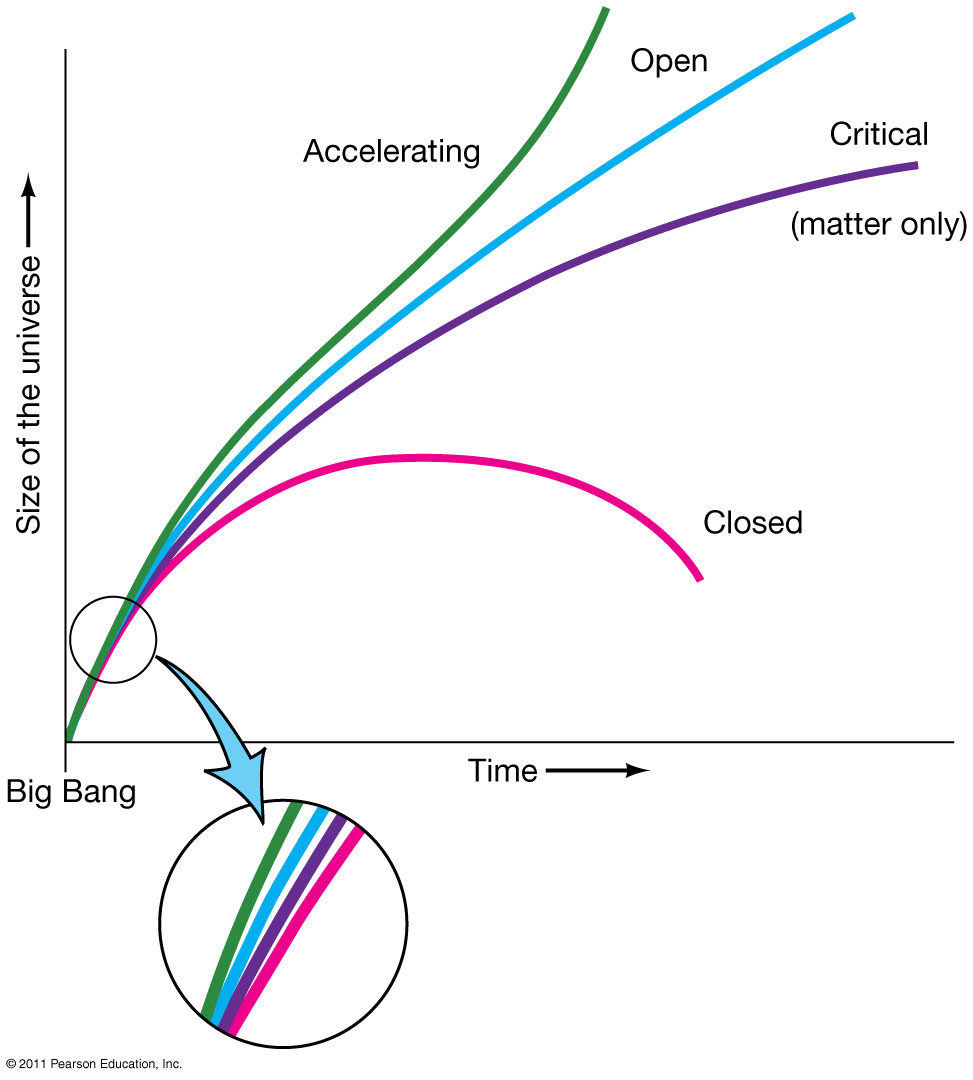
\includegraphics[keepaspectratio=true,scale=0.55]{flatnessProblem}}}
\captionof{figure}{A plot showing the evolution of the universe with time for different case of the spatial curvature parameter (taken from \url{http://physics.uoregon.edu/~jimbrau/BrauImNew/Chap27/7th/AT_7e_Figure_27_10.jpg}).}%      only if needed
\label{Fig2.1}
\end{minipage}

\subsection{The Horizon Problem}\label{subsec:HorProb}

In cosmology there also exists a particle horizon, which corresponds with the furthest distance from an observer that light moving along with the expansion of the universe could have travelled. This basically defines a sphere if we imagine every direction light could have travelled from some stationary observer. However the horizon problem reveals itself when we look in opposite directions on this surface and relates to the cosmological principle used when defining the FRW metric in equation (\ref{eq2.1}). Observations of the CMB reveal that the temperature is 2.726K \cite{Mather:1993ij} on either ends of the sphere despite the fact that causality prevents these regions from ever being able to interact with one another. This breaks causality because the universe was approximately 300,000 years old when the CMB was emitted. In addition to this, there are also very small fluctuations in the microwave background which would not be there without having been in causal contact. Once again, we may illustrate this problem with figure \ref{Fig2.2} below where `our galaxy' represents the stationary observer and points A and B are disconnected points each with their own Hubble sphere.

\noindent%
\begin{minipage}{\linewidth}% to keep image and caption on one page
\makebox[\linewidth]{%        to center the image
  \fbox{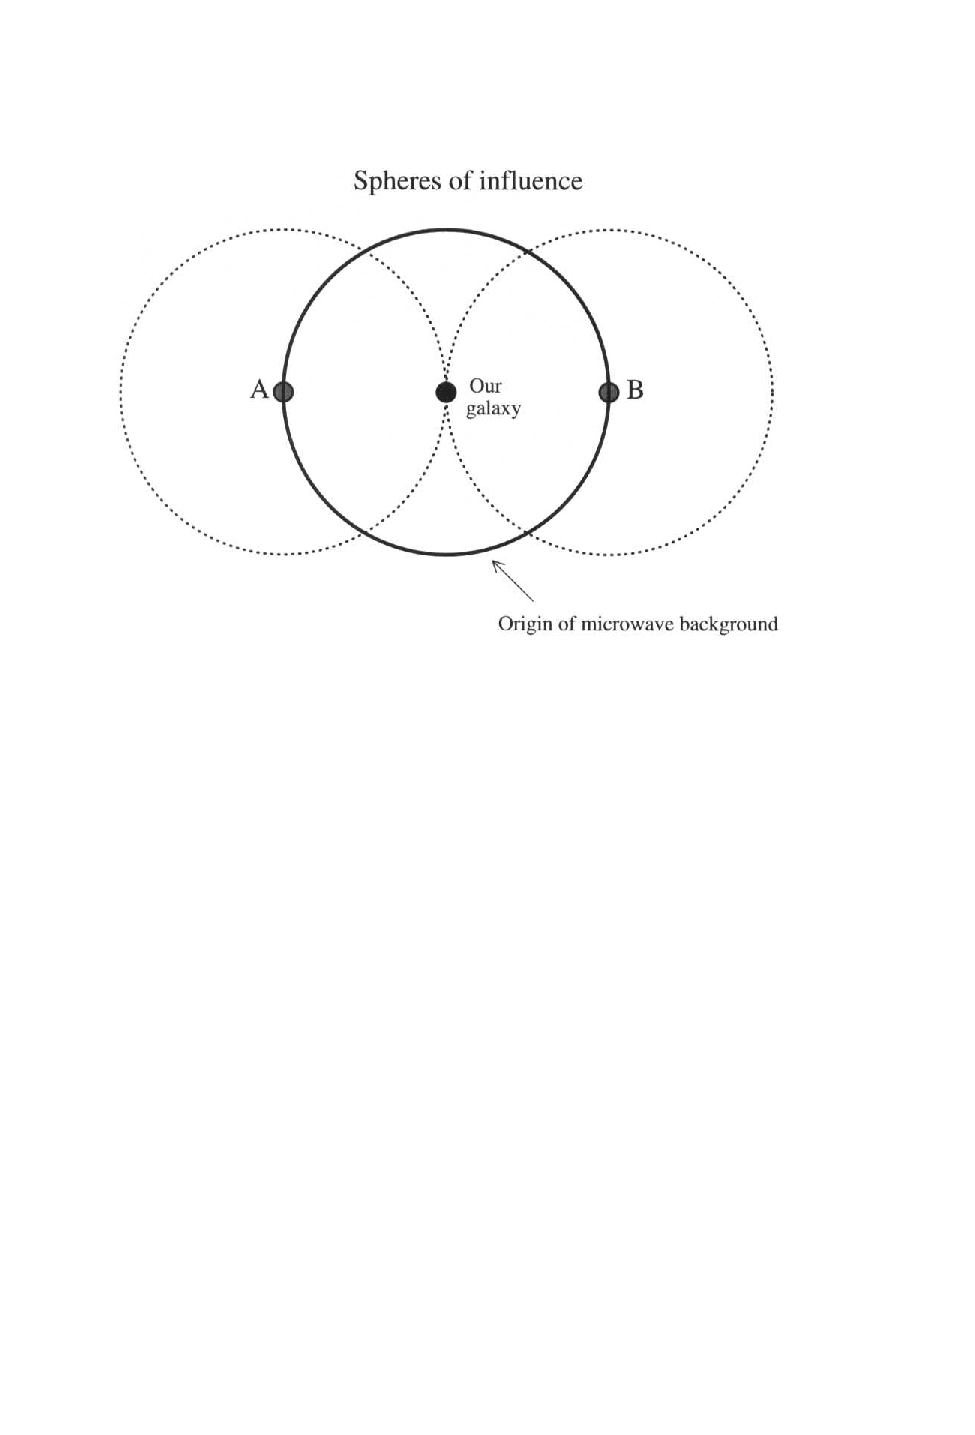
\includegraphics[keepaspectratio=true,scale=0.8]{HorizonProblem}}}
\captionof{figure}{A diagram showing two points A and B that are on opposite points of the sky and are causally disconnected (figure 13.1 from \cite{liddle2013introduction}).}%      only if needed
\label{Fig2.2}
\end{minipage}

\subsection{The Relics Problem}\label{subsec:RelicProb}

The third and final major problem with the $\Lambda$CDM model is the simplest one to understand but is perhaps the most important in the context of modern particle physics studies. Today, many of the models used in particle physics that go beyond the standard model predict new particles such as magnetic monopoles. However these particles only appear where the energies are so high that they cause the fundamental forces to be unified at the Grand Unified Scale (GUT) at about $10^{16}$ GeV. Energies this high can only exist in the very early universe where many of these particles would have been produced. As we observe none of these particles or their effects today, we can only conclude that the standard cosmological model is inconsistent with these GUT theories in its current form.

\section{Conditions for Inflation} \label{sec:CondInflation}

In 1981, inflation was originally proposed by Alan Guth \cite{Guth:1980zm} as a solution to these problems we have identified in the previous section. It is defined as being an initial time period in the early universe with an accelerating, almost exponential expansion rate $\dot{a}$ which essentially means that gravity was repulsive then. As we will later see, we also require that the observable universe was well inside the comoving Hubble radius at the beginning of inflation before transitioning to the outside of the radius by the end of inflation. Before that, we will establish some conditions for inflation using some of the Friedmann equations found in section \ref{sec:FriEqs}. If the rate of expansion is accelerating then it must be positive allowing us to give the first condition as:

\begin{equation}
\ddot{a} > 0. \label{eq2.5}
\end{equation}

If we insert the above condition into the second Friedmann equation (\ref{eq2.2b}), we realise that this gives the following condition on the energy density and pressure:

\begin{equation}
\rho + 3P < 0 \implies P < - \frac{\rho}{3}. \label{eq2.6}
\end{equation}

From equation (\ref{eq2.6}), we realise that that inflation must be generated by a negative pressure as the energy density $\rho$ is always positive. Fortunately, we will see in the next section that scalar fields can behave with a negative pressure and hence providing a generator for inflation.

We may also rewrite equation (\ref{eq2.5}) by realising that the Hubble radius $(aH)^{-1}$ is equivalent to $(\dot{a})^{-1}$ from the definition of the Hubble parameter. We can then relate the time derivative of the Hubble radius to $\ddot{a}$ and remove any terms that are always positive or constant to find:

\begin{equation}
\frac{d}{dt}\left(\frac{1}{aH}\right) < 0. \label{eq2.7}
\end{equation}

This tells us that the condition for inflation makes the comoving Hubble radius become smaller in size throughout inflation. However there are no constraints on the physical scale of the universe which is the vital property of inflation that allows it to solve the problems with the cosmological model. 

\subsection{Solution of the Flatness Problem} \label{subsec:FlatSol}

If we recall the first Friedmann equation used when defining the flatness problem earlier:

\begin{equation}
\frac{k}{(aH)^{2}} = \frac{\rho}{3M_{Pl}^{2}H^{2}} - 1, \label{eq2.8}
\end{equation}

we see that the inflationary condition found in equation (\ref{eq2.7}) causes the left hand side of the equation to decrease in size during inflation and will tend to zero given enough time. In fact, it can be shown \cite{lyth2009primordial} that inflation must increase the size of the universe by $\sim$50-60 e-folds by assuming inflation is followed by a reheating period before a radiation and then matter dominated universe to determine the evolution of the scale factor and combine those with observations from the CMB today. The solution to the flatness problem is shown in figure \ref{Fig2.3} below where the logarithm of the density parameter ($\Omega = \rho/(3M_{Pl}^{2}H^{2})$ here) is shown tending to zero during inflation giving a spatially flat universe at the end.

\noindent%
\begin{minipage}{\linewidth}% to keep image and caption on one page
\makebox[\linewidth]{%        to center the image
  \fbox{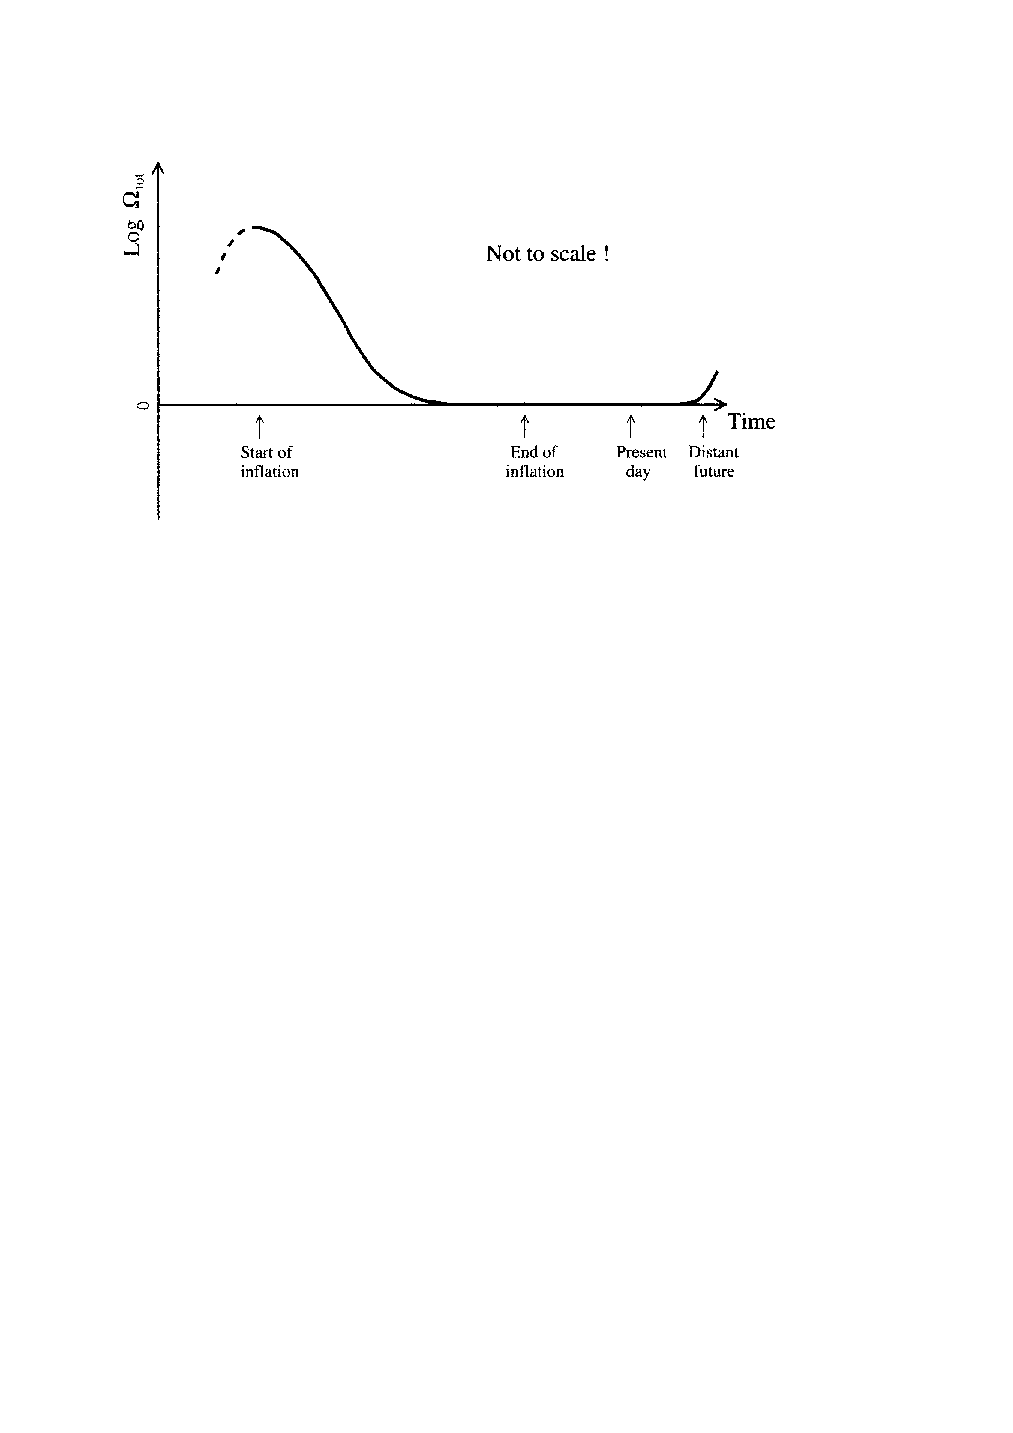
\includegraphics[keepaspectratio=true,scale=1]{FlatSol}}}
\captionof{figure}{A plot showing the logarithm of the density parameter $\Omega$ being driven towards zero during inflation (figure 13.2 from \cite{liddle2013introduction}).}%      only if needed
\label{Fig2.3}
\end{minipage}

\subsection{Solution of the Horizon Problem} \label{subsec:HorSol}

The last inflationary condition (\ref{eq2.7}) involving the Hubble radius also provides the solution to the horizon problem. As mentioned at the end of section \ref{sec:CondInflation}, equation (\ref{eq2.7}) provides no constraints on physical scales which means that scales within the Hubble radius can leave the horizon at a time known as the epoch of horizon exit. This solves the horizon problem because the causally disconnected homogeneous scales we observe today would have been causally connected if we assume they were all within the Hubble radius before inflation where the time these scales re-entered the horizon is the epoch of horizon re-entry. We can see all of these features as well as a plot of the comoving scales in figure \ref{Fig2.4} below.

\noindent%
\begin{minipage}{\linewidth}% to keep image and caption on one page
\makebox[\linewidth]{%        to center the image
  \fbox{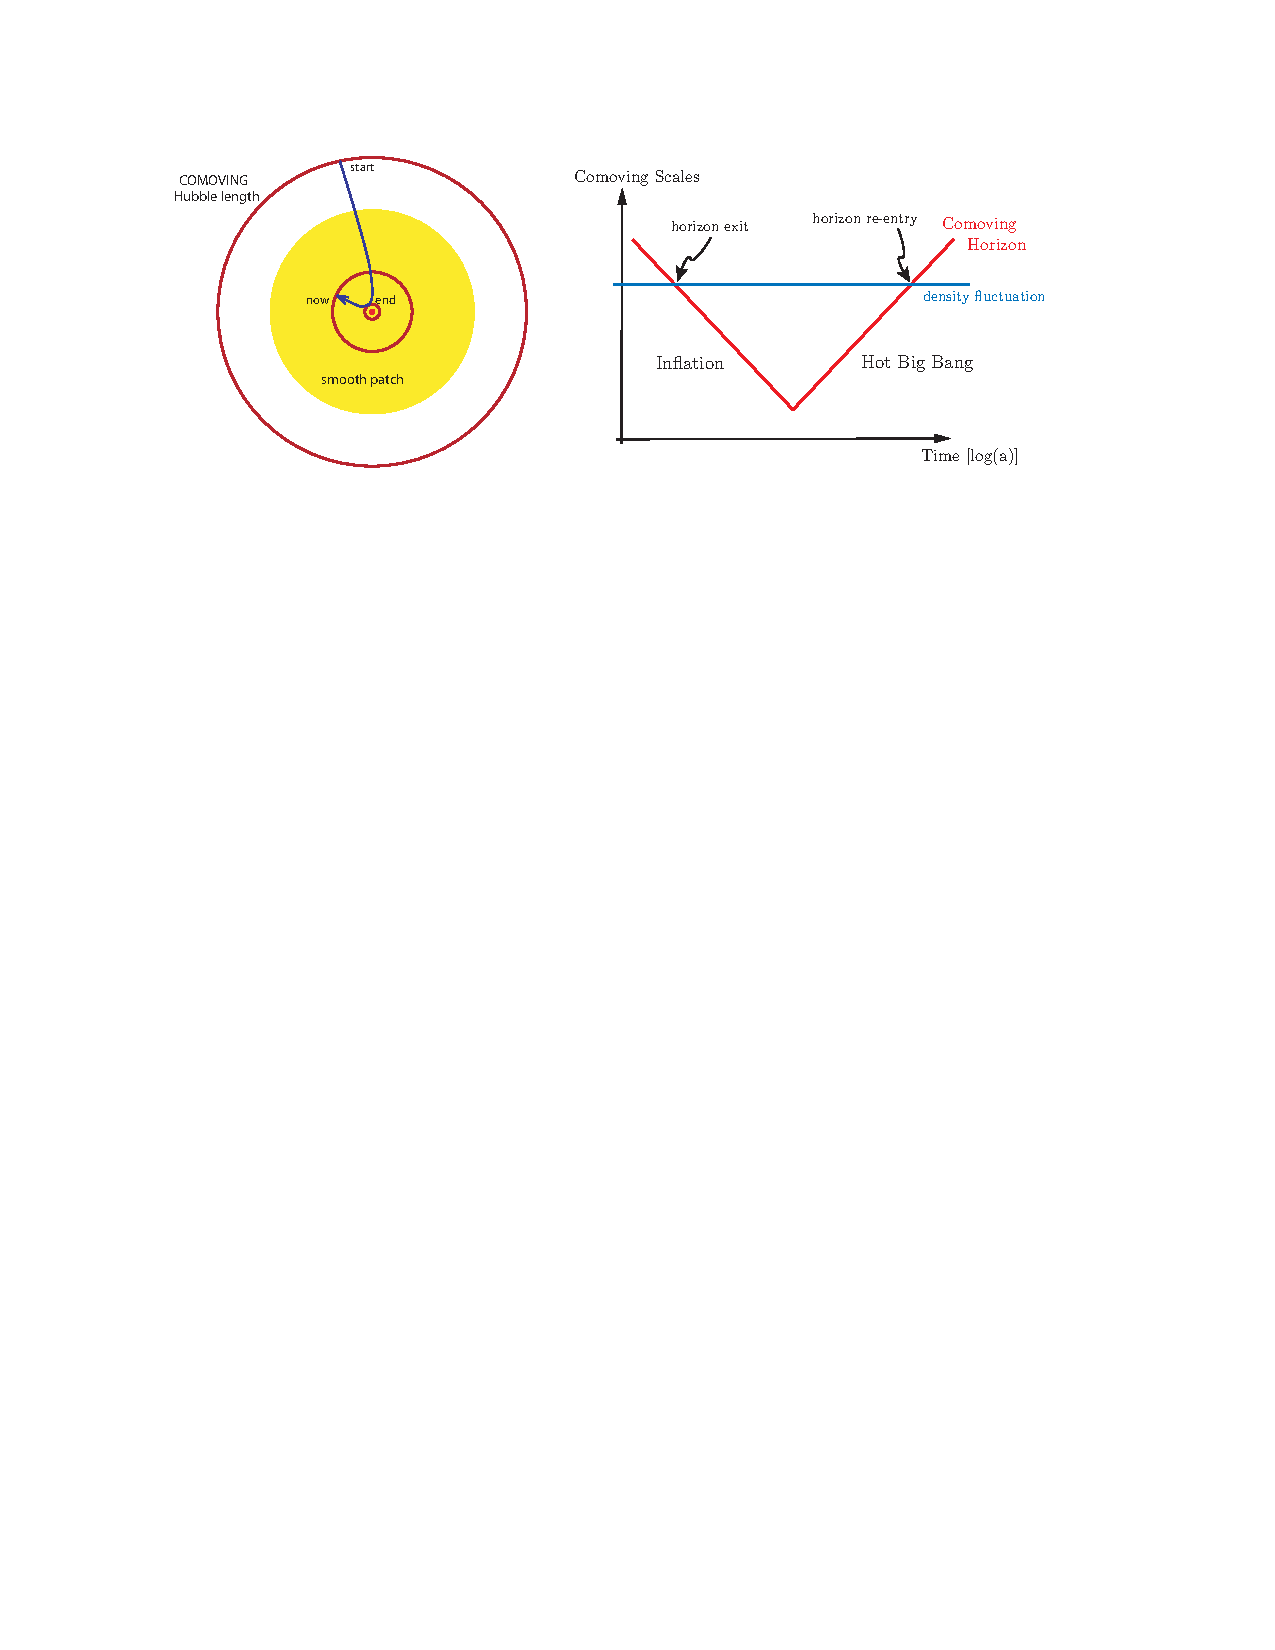
\includegraphics[keepaspectratio=true,scale=1.05]{HorizonSol}}}
\captionof{figure}{The left image shows the Hubble radius shrinking during inflation before expanding afterwards leaving the smooth patch. The right image shows a plot of this comoving horizon against time. (figure 4 from \cite{Baumann:2009ds}).}%      only if needed
\label{Fig2.4}
\end{minipage}

As we can see, the left image shows the physical scale in yellow exiting the horizon before increasing amounts of it begin re-entering the horizon after inflation leaving a homogeneous and isotropic patch afterwards.

\subsection{Solution of the Relics Problem} \label{subsec:RelicProblem}

The solution to the relics problems is the easiest one to understand and arises due to the rapid expansion of the universe causing the density of these proposed GUT particles. As these particles are produced at such high energies, they would have been the first ones to have been produced and hence would have left the horizon first on the very largest physical scales as well. This means less expansion is needed than is needed for the solutions to the flatness and horizon problems so the 50-60 e-folds of inflation will solve this problem too. There is only one other caveat and that is there is also a requirement that after inflation, the energy scale of the universe must be low enough so that no more of these exotic particles can be produced.

\section{Inflation Driven by a Scalar Field} \label{sec:InflatScalFields}

Now that we have established the requirements needed from inflation to solve the three major problems with the $\Lambda$CDM model, we must now introduce scalar fields as a means of generating inflation and show why it satisfies our conditions found in the previous section. We will begin with an overview of what a scalar field as well as how to describe it using Lagrangian mechanics before deriving an equation of motion for the scalar field in a curved spacetime with solutions that satisfy our inflationary conditions. 

\subsection{What is a Scalar Field?}

Classically, a scalar field is a field whose value is invariant under a Lorentz transformation (rotation) of the coordinate system which can be written as:

\begin{equation}
\phi^{\prime}\left(x^{\prime}, y^{\prime}, z^{\prime} \right) = \phi \left(x, y, z \right). \label{eq2.9}
\end{equation}

An example of a classical scalar field would be the temperature of a fluid or the gravitational potential. In quantum field theory, each type of field corresponds with a type of elementary particle where the scalar field corresponds with all spin-0 particles like for example the Higgs boson and field which determines the masses of elementary particles. It is believed that the value of the scalar fields is the dominant effect on the dynamics of the early universe which is one reason it is a suitable candidate for inflation. It is also possible for a scalar field to have changed its value significantly in the time since the inflationary period which would explain why we no longer see its effect. 

\subsection{Lagrangian Mechanics} \label{subsec:LagMechs}

In order to allow us to describe the dynamics of a scalar field, we must introduce several important quantities used in classical field theory. In Lagrangian mechanics, the physics of a problem is all contained within Lagrangians and actions where we first introduce the Lagrangian, $L(x, \dot{x}, t)$ as:

\begin{equation}
L(x, \dot{x}, t) = T(\dot{x}, t) - V(x, t) = \int \mathcal{L}(x, \dot{x}, t) \hspace{2pt} d^{3}x, \label{eq2.10}
\end{equation}

where we have introduced a kinetic energy term $T$, a potential energy term $V$ and a Lagrangian density $\mathcal{L}(x, \dot{x}, t)$. We also have actions which are defined in terms of the Lagrangian density as:

\begin{equation}
S = \int \mathcal{L}(x, \dot{x}, t) \hspace{2pt} d^{4}x. \label{eq2.11}
\end{equation}

Finally, the action principle ($\delta S = 0$) uses calculus of variations on $x$ and $\dot{x}$ \cite{kibble2004classical} to find the Euler-Lagrange equation which gives an equation of motion for the Lagrangian as:

\begin{equation}
\frac{\partial L}{\partial x} - \frac{\partial}{\partial t}\left(\frac{\partial L}{\partial \dot{x}} \right) = 0. \label{eq2.12}
\end{equation}

\subsection{Scalar Fields in a Curved Spacetime} \label{subsec:ScalFieldsCurvST}

We must first consider some Lagrangian density that is invariant under a Lorentz transformation, obeys the relativistic energy momentum relation ($E^{2} = m^{2} + \abs{\vec{p}}^{2}$) and is in terms of a scalar field denoted by $\phi$. Using these motivations \cite{mandl2010quantum}, we realise that the simplest form for the Lagrangian density is given by:

\begin{equation}
\mathcal{L} = -\frac{1}{2}\partial^{\mu} \phi \partial_{\mu}\phi - V(\phi), \label{eq2.13}
\end{equation}

where $\partial_{\mu}$ is a derivative over all four components of spacetime and $\partial^{\mu} \equiv g^{\mu \nu}\partial_{\nu}$. The action associated with this Lagrangian density is then given by:

\begin{equation}
S = \int d^{4}x \hspace{2pt} \sqrt{-g} \hspace{2pt} \mathcal{L}, \label{eq2.14}
\end{equation}

where $g$ is given by $\det(g_{\mu \nu})$ and appears because of the coordinate transform to the spacetime volume element defined on the constant hypersurface. If we were going to use the flat spacetime metric tensor, $\eta_{\mu \nu}$, we would find the above action gives the Klein-Gordon equation when using the Euler-Lagrange equation in (\ref{eq2.12}). In principle, we could do the same thing with our spacetime metric defined in equation (\ref{eq2.1}) to find an equation of motion for a scalar field in a curved spacetime. However it is more useful to find relations for energy density and pressure so that we can use them in the Friedmann equations from section \ref{sec:FriEqs} and place some constraints on inflation in terms of the scalar field. This is done using the stress-energy tensor equation for a flat universe where $k = 0$ which yields the following for the Lagrangian density above:

\begin{equation}
\begin{aligned} \label{eq2.15}
\tensor{T}{^{\mu \nu}} &= \tensor{\partial}{^{\mu}}\phi \tensor{\partial}{^{\nu}}\phi - \tensor{g}{^{\mu \nu}} \mathcal{L} \\
&= \tensor{\partial}{^{\mu}}\phi \tensor{\partial}{^{\nu}}\phi - \tensor{g}{^{\mu \nu}} \left[\frac{1}{2} \left(\partial_{\sigma}\phi\right)\left(\partial^{\sigma}\phi \right) - V(\phi) \right].
\end{aligned}
\end{equation} 

If we now assume that the scalar field behaves like a perfect fluid so that it has no shear stresses, viscosity or heat conductivity and that the scalar field is homogeneous with no spatial derivatives, we can first find the energy density as:

\begin{equation} \label{eq2.16}
\begin{aligned}
\rho &= \tensor{T}{^{00}} \\
&= \frac{1}{2} \dot{\phi}^{2} + V(\phi),
\end{aligned}
\end{equation}

and the pressure as:

\begin{equation} \label{eq2.17}
\begin{aligned}
P &= \frac{1}{3} \sum\limits_{i=1}^{3} T^{ii} \\
&= \frac{1}{2} \dot{\phi}^{2} - V(\phi).
\end{aligned}
\end{equation}

We can get an equation of motion for our scalar field by placing equations (\ref{eq2.16}) and (\ref{eq2.17}) into the energy conservation expression in equation (\ref{eq2.3}) to find:

\begin{equation} \label{eq2.18}
\ddot{\phi} + 3H\dot{\phi} +V^{\prime}(\phi) = 0,
\end{equation}

where over-dots indicate a derivative with respect to physical time and primes indicates a derivative with respect to $\phi$. As we can see, if the potential is constant, this is the equation for a damped harmonic oscillator where the damping term is $3H\dot{\phi}$ and is known as Hubble damping. If the potential dominates over the damping term instead, we have a solution that decays exponentially according to the value of the potential. We can find out which situation is better suited for inflation by substituting the energy density and pressure solutions into the Friedmann equations (\ref{eq2.2a}) and (\ref{eq2.2b}) with $k = 0$ to find:

\begin{subequations}
\begin{align}
H^{2} &= \frac{1}{3M_{Pl}^{2}}\left( \frac{1}{2} \dot{\phi}^{2} + V(\phi) \right), \label{eq2.19a} \\
\frac{\ddot{a}}{a} &= - \frac{1}{3M_{Pl}^{2}} \left(\dot{\phi}^{2} - V(\phi)\right). \label{eq2.19b}
\end{align}
\end{subequations}

The first condition we gave for inflation is that $\ddot{a} > 0$ which from equation (\ref{eq2.19b}), we see that $V(\phi)$ must be much larger than $\dot{\phi}^{2}$ for this to make the right hand side of the equation positive and satisfy the condition. As the other conditions (\ref{eq2.6}) and (\ref{eq2.7}) are derived from the second Friedmann equation, we see that $V(\phi) \gg \dot{\phi}^{2}$ also gives the negative pressure needed as well as the horizon crossing properties for inflation as well. All of this implies that during inflation, we should see that the solution of the equation of motion (\ref{eq2.18}) is the exponentially decaying solution mentioned earlier where the other damped oscillator solution is associated with the reheating epoch that begins after inflation is finished.

\section{The Slow-roll Approximation} \label{sec:SlowRollApprox}

Equation (\ref{eq2.18}) is a second order differential equation in $\phi$ that needs initial conditions for a solution and in this section we'll see how the condition $V(\phi) \gg \dot{\phi}^{2}$ can be used to form some parameters known as the slow-roll parameters that can give initial conditions in $\phi$ and $V(\phi)$.

\subsection{Defining the First Slow-roll Parameter} \label{subsec:DefFirstSparam}

We will begin by defining a parameter $\epsilon$ by using the condition $\ddot{a}/a > 0$ and rewriting it in terms of $H$ from $H = \dot{a} / a$ to give the following expression:

\begin{equation} \label{eq2.20}
\frac{\ddot{a}}{a} = H^{2} + \dot{H} > 0 \implies \epsilon \equiv - \frac{\dot{H}}{H^{2}} < 1.
\end{equation}

Next we can differentiate equation (\ref{eq2.19a}) with respect to time and rewrite it so that it can be compared with the scalar field equation of motion as:

\begin{equation} \label{eq2.21}
\ddot{\phi} + 3H\dot{\phi} \left(-\frac{2M_{Pl}^{2}}{\dot{\phi}^{2}} \dot{H} \right) + V^{\prime}(\phi) = 0.
\end{equation}

As we can see this is identical to the field equation (\ref{eq2.18}) if the term in brackets is equal to one which can be achieved by setting $\dot{H}$ as:

\begin{equation} \label{eq2.22}
\dot{H} = - \frac{\dot{\phi}^{2}}{2 M_{Pl}^{2}}.
\end{equation}

Therefore we can write the parameter $\epsilon$ as:

\begin{equation} \label{eq2.23}
\epsilon = - \frac{\dot{H}}{H^{2}} = \frac{\dot{\phi}^{2}}{2 M_{Pl}^{2} H^{2}}.
\end{equation}

All of these expressions are exact so far but we can rewrite $\epsilon$ in terms of potentials by using the condition $V(\phi) \gg \dot{\phi}^{2}$. If we take time derivatives of the condition, we realise that $V'(\phi) \gg \ddot{\phi}$ also holds true which means we can approximate equations (\ref{eq2.18}) and (\ref{eq2.19a}) as:

\begin{subequations}
\begin{align}
3H\dot{\phi} &\approx V^{\prime}(\phi), \label{eq2.24a} \\
H^{2} &\approx \frac{V(\phi)}{3M_{Pl}^{2}}. \label{eq2.24b}
\end{align}
\end{subequations}

If we now substitute equations (\ref{eq2.24a}) and (\ref{eq2.24b}) into equation (\ref{eq2.23}), we find:

\begin{equation} \label{eq2.25}
\epsilon \approx \frac{M_{Pl}^{2}}{2} \left(\frac{V^{\prime}(\phi)}{V(\phi)}\right)^{2} \ll 1.
\end{equation}

This is the first slow-roll parameter and the approximations used form the basis of the slow-roll approximation where the slow-roll part comes from the requirement that the field `rolls' very slowly compared with the potential.

\subsection{More Slow-roll Parameters} \label{subsec:MoreSrollPars}

We can repeat this process by first differentiating equation (\ref{eq2.24a}) in $\phi$ and comparing with the field equation (\ref{eq2.18}) again \cite{lyth2009primordial} to obtain the second slow-roll parameter $\eta$ as: 

\begin{equation} \label{eq2.26}
\eta \approx M_{Pl}^{2} \frac{V^{\prime \prime}(\phi)}{V(\phi)} \ll 1.
\end{equation}

For our discussion of the perturbations caused by inflation later, we also give two higher order slow-roll parameters \cite{lyth2009primordial} as:

\begin{subequations}
\begin{align}
\xi &\approx M_{Pl}^{4} \frac{V^{\prime}(V^{\prime \prime \prime})}{V^{2}}, \label{eq2.27a} \\
\sigma &\approx M_{Pl}^{6} \frac{(V^{\prime})^{2}(V^{\prime \prime \prime \prime})}{V^{3}}. \label{eq2.27b}
\end{align}
\end{subequations}

\subsection{Number of e-folds} \label{subsec:NoEfolds}

We can now find expressions for the initial and final conditions in $\phi$ so that inflation can last for approximately 50-60 e-folds as required to solve the flatness and horizon problems. If we first define the scale factor during inflation to be exponentially increasing according to the Hubble parameter with time as $a(t) = e^{Ht}$ and define an e-fold to be the time taken for the scale factor to increase in size by a factor of $e$, then we can write:

\begin{equation} \label{eq2.28}
N(\phi) = \ln \left(\frac{a_{end}}{a_{0}}\right) = \int_{t_{0}}^{t_{end}} H dt = \int_{\phi_{0}}^{\phi_{end}} \frac{H}{\dot{\phi}} d\phi,
\end{equation}

where there has been a change in variables from $t$ to $\phi$ and $a_{0}$ has been normalised to one here. From equation (\ref{eq2.23}), we realise this can be written in terms of the first slow-roll parameter as:

\begin{equation} \label{eq2.29}
N(\phi) = \int_{\phi_{0}}^{\phi_{end}} \frac{H}{\dot{\phi}} d\phi = \frac{1}{M_{Pl}} \int_{\phi_{0}}^{\phi_{end}} \frac{1}{\sqrt{2\epsilon}} d\phi \approx \frac{1}{M_{Pl}^{2}} \int_{\phi_{0}}^{\phi_{end}} \frac{V(\phi)}{V^{\prime}(\phi)} d\phi.
\end{equation}

We may define $\phi_{end}$ using the first slow-roll parameter as being the value of $\phi$ where the slow-roll approximation is no longer fulfilled as:

\begin{equation} \label{eq2.30}
\epsilon(\phi_{end}) \approx \frac{M_{Pl}^{2}}{2} \left(\frac{V^{\prime}(\phi_{end})}{V(\phi_{end})}\right)^{2} = 1.
\end{equation}

Therefore if we solve equation (\ref{eq2.30}) for $\phi_{end}$ and substitute it into equation (\ref{eq2.29}) with $50 \le N(\phi) \le 60$, we can find the initial $\phi_{0}$ needed to solve equation (\ref{eq2.18}) for the `right' amount of inflation needed. As we will see in the later theory sections, the slow-roll parameters can be used to parametrise other aspects of inflation such as the fluctuations caused by the field quantisation.

\section{Inhomogeneities from Inflation} \label{sec:InhomoInflat}

So far, we have only considered inflation for the case where neither the scalar field $\phi$ or the spacetime metric tensor $g_{\mu \nu}$ are perturbed so that there are no inhomogeneities. However, cosmological perturbation theory can be used to find classical fluctuations in the scalar field and derive equations to describe them. Initially, we will describe the perturbations in the spacetime metric and show how they can be decomposed into scalar, vector and tensor modes as well as giving expressions for the matter and scalar field perturbations. Next, we will introduce some gauge-invariant variables to describe the curvature perturbations produced which allow the perturbations in the scalar field to be written only in terms of these gauge-invariants. Finally, we will give some statistical measures for the gauge-invariants to use when we later derive an equation of motion for the quantised perturbations.

\subsection{Perturbations in the Spacetime Metric} \label{CosPertTh}

We shall begin by introducing a new conformal time variable $\tau$ that tracks the time taken for a photon to travel from the furthest distance caused by expansion and is given by:

\begin{equation} \label{eq2.31}
\tau = \int_{0}^{t} \frac{dt^{\prime}}{a(t^{\prime})} = \int_{0}^{a} \mathrm{d}\ln a^{\prime} \frac{1}{a^{\prime} H} = \int_{0}^{a} \frac{da^{\prime}}{(a^{\prime})^{2} H} \approx -\frac{1}{aH}.
\end{equation}

This allows the FRW spacetime line element defined in equation (\ref{eq2.1}) to be rewritten as \cite{Baumann:2009ds}: 

\begin{equation} \label{eq2.32}
ds^{2} = a^{2}(\tau) \left[-d\tau^{2} + \gamma_{ij}dx^{i}dx^{j} \right],
\end{equation}

where we have assumed isotropy and $\gamma_{ij}$ is the 3D spatial metric on the constant $\tau$ hypersurface and is defined as:

\begin{equation} \label{eq2.33}
\gamma_{ij} = \frac{\delta_{ij}}{\left[1 + \frac{1}{4} k(x^2 + y^2+ z^2) \right]^{2}}.
\end{equation}

Next we may define a perturbed spacetime line element \cite{Mukhanov:1990me} which is written in the following form :

\begin{equation} \label{eq2.34}
ds^{2} = \tensor*{g}{^{(0)}_\mu_\nu} dx^{\mu} dx^{\nu} + \delta \tensor{g}{_{\mu \nu}} dx^{\mu} dx^{\nu},
\end{equation}

where the new spacetime metric tensor has been decomposed into:

\begin{equation} \label{eq2.35}
\tensor{g}{_{\mu \nu}} = \tensor*{g}{^{(0)}_\mu_\nu} + \delta \tensor{g}{_{\mu \nu}},
\end{equation}

with $\tensor*{g}{^{(0)}_\mu_\nu}$ representing the unperturbed spacetime metric tensor and $\delta \tensor{g}{_{\mu \nu}}$ gives its perturbation. It is now helpful to split this perturbation into scalar, vector and tensor components \cite{Mukhanov:1990me, Langlois:2004de, Weinberg:2008zzc} where the classification refers to the way each one transforms the spatial components on the comoving hypersurface. It can be shown \cite{Baumann:2009ds} using rotational and translational invariance that independent Fourier modes of these components are independent allowing us to treat them separately. This is important because each component has a different physical significance where the scalar perturbations give inhomogeneities in the field which can cause differences in the density of matter. Also the tensor perturbations give arise to gravitational waves which we will find out may be observable in space missions such as Planck or BICEP. The vector perturbations are not produced by a scalar field and decay very quickly so lead to no observable effects for us to calculate here.

\subsubsection{Scalar Modes} \label{subsubsec:ScalModes}

If we first assume a spatially flat universe ($k = 0$) so that $\gamma_{ij} = \delta_{ij}$, then we may write the most general form \cite{Mukhanov:1990me, Langlois:2004de, Baumann:2009ds, lyth2009primordial, Weinberg:2008zzc} for the scalar metric perturbations as:

\begin{equation} \label{eq2.36}
\delta g_{\mu \nu} = - a^{2}(\tau) \begin{pmatrix}
	2\Phi & -B_{,i} \\[0.3em]
	-B_{,i} & 2(\Psi \delta_{ij} - E_{,ij}) \\[0.3em]
\end{pmatrix},
\end{equation}

where $\Phi$, $B$, $\Psi$ and $E$ are all scalar quantities that are functions of the spacetime coordinates and a comma index indicates a partial derivative with respect to the next coordinate index. By using equations (\ref{eq2.32}), (\ref{eq2.35}) and (\ref{eq2.36}) in equation (\ref{eq2.34}), we find that the form  of the line element in the scalar metric perturbations \cite{Mukhanov:1990me, Langlois:2004de, Baumann:2009ds, lyth2009primordial, Weinberg:2008zzc} to be:

\begin{equation} \label{eq2.37}
ds^{2} = a^{2}(\tau)\left[-(1+2\Phi)d\tau^{2} + 2B_{,i}dx^{i}d\tau + \{(1 - 2\Psi)\delta_{ij} + 2E_{,ij}\}dx^{i}dx^{j} \right].
\end{equation}

However under a coordinate transformation, the scalar fluctuations change so in order to make our scalar metric perturbations invariant, we introduce the following gauge transformation:

\begin{subequations}
\begin{align}
t &\rightarrow t + \alpha, \label{eq2.38a} \\
x^{i} &\rightarrow x^{i} + \delta^{ij}\beta_{,j}. \label{eq2.38b}
\end{align}
\end{subequations}

This means our scalar metric perturbations now transform as:

\begin{subequations}
\begin{align}
\Phi &\rightarrow \Phi - \dot{\alpha}, \label{eq2.39a} \\
B &\rightarrow B + a^{-1}\alpha - a\dot{\beta}, \label{eq2.39b} \\
E &\rightarrow E - \beta, \label{eq2.39c} \\
\Psi &\rightarrow \Psi + H\alpha. \label{eq2.39d}
\end{align}
\end{subequations}

\subsubsection{Tensor Modes} \label{subsubsec:TensModes}

The most general form of the tensor metric perturbations can be simply written as:

\begin{equation} \label{eq2.40}
\delta g_{\mu \nu} = a^{2}(\tau) \begin{pmatrix}
0 & 0 \\[0.3em]
0 & h_{ij}
\end{pmatrix},
\end{equation}

where $h_{ij}$ is 2-rank tensor perturbation. Equations (\ref{eq2.32}), (\ref{eq2.35}) and (\ref{eq2.40}) can be used in equation (\ref{eq2.34}) to give a spacetime line element:

\begin{equation} \label{eq2.41}
ds^{2} = a^{2}(\tau) \left[-d\tau^{2} + (\delta_{ij} + h_{ij})dx^{i}dx^{j} \right]
\end{equation}

No gauge transformation is needed for the tensor modes as they are invariant under a coordinate transform.

\subsection{Stress-Energy Perturbations} \label{StreEnePerturb}

Inflationary energy is the biggest contributor to the stress-energy tensor during the early universe so that perturbations in the scalar field give perturbations on the stress energy tensor. Therefore we can write the perturbed stress-energy tensor for the cosmological fluid representing the matter as:

\begin{subequations} \label{eq2.42}
\begin{align}
\tensor*{T}{_0^0} &= -(\rho^{(0)} + \delta \rho), \label{eq2.42a} \\
\tensor*{T}{_i^0} &= (\rho^{(0)} + P^{(0)})v_{i}, \label{eq2.42b} \\
\tensor*{T}{_0^i} &= -(\rho^{(0)} + P^{(0)})(v^{i} + B^{i}), \label{eq2.42c} \\
\tensor*{T}{^i_j} &= \tensor*{\delta}{^i_j}(P^{(0)} + \delta P) + \tensor*{\Sigma}{^i_j}, \label{eq2.42d}
\end{align}
\end{subequations}

where $v^{i}$ is a three dimensional fluid velocity, $\Sigma$ is the anisotropic stress and the index $(0)$ represents the unperturbed densities and pressures. Only the anisotropic stress is gauge-invariant here so we can write transformations of the energy density, pressure and momentum density ($q^{(0)}_i \equiv (\rho^{(0)} + P^{(0)})v_{i})$ using our gauge transformation above as:

\begin{subequations}
\begin{align}
\delta \rho &\rightarrow \delta \rho - \dot{\rho^{(0)}} \alpha, \label{eq2.43a} \\
\delta P &\rightarrow \delta P - \dot{P^{(0)}} \alpha, \label{eq2.43b} \\
\delta q &\rightarrow \delta q + (\rho^{(0)} + P^{(0)}) \alpha. \label{eq2.43c}
\end{align}
\end{subequations}

\subsubsection{Scalar Field Perturbations} \label{subsubsec:ScalFieldPerturbs}

As we already have equation (\ref{eq2.15}) that gives a relation between the scalar field $\phi$, we may define the perturbed scalar field $\phi = \phi^{(0)} + \delta \phi$ and use equation (\ref{eq2.42}) with the metric perturbations to find:

\begin{subequations}
\begin{align}
\tensor*{T}{_0^0} &= \delta \rho = -\dot{\phi}\dot{\delta \phi} - \dot{V}\delta \phi + \dot{\phi}^{2}\Phi, \label{eq2.44a} \\
\tensor*{T}{_i^0} &= \partial_{i} \delta q = -\dot{\phi^{(0)}}\partial_{i}\delta\phi, \label{eq2.44b} \\
\tensor*{T}{_0^0} &= \tensor*{\delta}{^i_j}\left( \dot{V} \delta \phi + \dot{\phi}^{2} \Phi - \dot{\phi} \dot{\delta \phi} \right) . \label{eq2.44c}
\end{align}
\end{subequations}

\subsection{Curvature Perturbations and Gauge-Invariance} \label{subsec:CurvPerturbsGaugeInvar}

In principle, one could use the Einstein equations in terms of all the perturbed variables we have found in the preceding sections and then find equations that describe the evolution the important perturbations that have left the horizon. Instead, we can avoid this by introducing gauge-invariant curvature perturbation variables \cite{Bardeen:1983qw, Weinberg:2008zzc, Langlois:2004de}. The first curvature parameter represents the curvature on constant density hypersurfaces, $R^{(3)} = 4 \nabla^{2}\Psi / a^{2}$, and is given by:

\begin{equation} \label{eq2.45}
-\zeta \equiv \Psi + \frac{H}{\dot{\rho^{(0)}}} \delta \rho.
\end{equation}

This variable is particularly useful because it remains constant after horizon crossing which allows its statistics to be used to tell us about the early universe.It is also gauge-invariant meaning that it can be used regardless of the gauge chosen for the perturbations. It can be given in terms of the scalar field during slow-roll inflation as:

\begin{equation} \label{eq2.46}
-\zeta \approx \Psi + \frac{H}{\dot{\phi^{(0)}}} \delta \phi.
\end{equation}

We can introduce another gauge-invariant invariable that gives the comoving curvature perturbation that instead defines the curvature on comoving constant density hypersurfaces as:

\begin{equation} \label{eq2.47}
\mathcal{R} = \Psi + \frac{H}{ \dot{\rho^{(0)}} + \dot{P^{(0)}} } \delta q .
\end{equation}

Equation (\ref{eq2.44b}) allows us to rewrite this as:

\begin{equation} \label{eq2.48}
\mathcal{R} = \Psi + \frac{H}{\dot{\phi^{(0)}}} \delta \phi, 
\end{equation}

where we see that $\zeta$ and $\mathcal{R}$ are equivalent during slow-roll inflation from equations (\ref{eq2.46}) and (\ref{eq2.48}). The Einstein equations can also be used to give a relation between these variables which is:

\begin{equation} \label{eq2.49}
-\zeta = \mathcal{R} + \left( \frac{k}{aH} \right)^{2} \frac{2 \rho^{(0)}}{3( \rho^{(0)} + P^{(0)})} \Psi_{B},
\end{equation}

where:

\begin{equation} \label{eq2.50}
\Psi_{B} \equiv \Psi + a^{2}H\left(\dot{E} - \frac{B}{a} \right).
\end{equation}

Therefore we see that $\zeta$ and $\mathcal{R}$ are also equal on super-horizon scales where $k \ll aH$ as well as being conserved after horizon crossing. This means that any statistical measures must also be computed after horizon crossing. The Bardeen potential, $\Psi_{B}$, is another gauge-invariant variable and corresponds with a curvature perturbation physically.

\subsection{Statistics of the Fluctuations} \label{subsec:StatFluc}

The inhomogeneities in the fluctuations of the scalar field are quantified using a power spectrum that determines the scale dependance for the power of the variations. We have shown that the perturbations can be written in terms of $\mathcal{R}$ (or $\zeta$) so we Fourier transform the components and perform an average over the ensemble of possible states as:

\begin{equation} \label{eq2.51}
\langle \mathcal{R}_{\vec{k}} \mathcal{R}_{\vec{k^{\prime}}} \rangle = (2 \pi)^{3} \delta(\vec{k} + \vec{k^{\prime}}) P_{\mathcal{R}}(k).
\end{equation}

We then define the dimensionless scalar power spectrum, $\Delta^{2}_{s}$, as:

\begin{equation} \label{eq2.52}
\Delta^{2}_{s} \equiv \Delta^{2}_{\mathcal{R}} = \frac{k^{3}}{2 \pi^{2}} P_{\mathcal{R}}(k),
\end{equation}

where the normalisation has been chosen so that $\langle \mathcal{R} \mathcal{R} \rangle = \int_{0}^{\infty} \Delta_{\mathcal{R}}^{2}(k) \mathrm{d}\ln k$. We can then define a scalar spectral index, $n_{s}$, that measures the scalar scale variance as:

\begin{equation} \label{eq2.53}
n_{s} - 1 \equiv \frac{d\ln \Delta^{2}_{s}}{d\ln k},
\end{equation}

where the convention is chosen such that $n_{s} = 1$ for scale invariance. In principle, the scalar power spectrum and spectral index should give all the information about the scalar fluctuations but we also need a measure of the tensor fluctuations. Equations (\ref{eq2.40}) and (\ref{eq2.41}) told us that the only quantity needed to describe the tensor modes is $h_{ij}$ which are polarised as $+$ and $\times$ modes. The ensemble average of the Fourier components of $h$ is defined as:

\begin{equation} \label{eq2.54}
\langle h_{\vec{k}} h_{\vec{k^{\prime}}} \rangle = (2 \pi)^{3} \delta(\vec{k} + \vec{k^{\prime}}) P_{h}(k).
\end{equation}

The dimensionless power spectrum of polarisation of the tensor modes, $\Delta^{2}_{h}$, is defined as:

\begin{equation} \label{eq2.55}
\Delta^{2}_{h} = \frac{k^{3}}{2 \pi^{2}} P_{h}(k),
\end{equation}

where the dimensionless tensor power spectrum, $\Delta^{2}_{t}$, is defined as the sum of the power spectrum for each polarisation:

\begin{equation} \label{eq2.56}
\Delta^{2}_{t} = 2 \Delta^{2}_{h} = \frac{k^{3}}{\pi^{2}} P_{h}(k).
\end{equation}

The tensor modes also have a tensor spectral index given by:

\begin{equation} \label{eq2.57}
n_{t} \equiv \frac{d\ln \Delta^{2}_{t}}{d\ln k},
\end{equation}

where scale-invariance in the tensor modes is given by $n_{t} = 0$ here.

\section{Quantising the Fluctuations} \label{sec:QuanFluc}

Now that we have found the parameters needed to describe the scalar and tensor inhomogeneities caused by inflation, we must now use the inflationary framework we found in section \ref{subsec:ScalFieldsCurvST} to write an equation of motion in terms of these new parameters. Then by quantising the field in the equation of motion, we can derive equations for the statistical measures we introduced at the end of the last section.

\subsection{Scalar Field Action} \label{subsec:ScalFieldAct}

We must now form an action for the scalar field so that we can rewrite it in terms of our curvature variable $\mathcal{R}$. This can be done by using the Lagrangian density formed in equation (\ref{eq2.13}) and couple it to gravity using the Einstein-Hilbert action \cite{hilbert1915grundlagen} to give the following action:

\begin{equation} \label{eq2.58}
S = \frac{1}{2} \int d^{4} x \sqrt{-g} \left[R - \partial_{\mu}\phi \partial^{\mu}\phi - 2V(\phi) \right],
\end{equation}

where $M_{Pl}^{2} = 1$ from now on. It is now possible to expand this action to second order in $\mathcal{R}$ by first writing the fluctuations in the ADM formalism \cite{Arnowitt:1962hi} before using the comoving gauge allowing all fluctuations to be written in terms of $\mathcal{R}$ \cite{Mukhanov:1990me, Maldacena:2002vr, Baumann:2009ds} and rewrite the action for scalar perturbations as:

\begin{equation} \label{eq2.59}
S_{(2)} = \frac{1}{2} \int d^{4}x \hspace{2pt} a^{3} \frac{\dot{\phi}^{2}}{H^{2}}\left[ \dot{\mathcal{R}}^{2} - \frac{(\partial_{i}\mathcal{R})^{2}}{a^{2}} \right]
\end{equation}

Next we can define the Mukhanov-Sasaki variable \cite{Mukhanov:1985rz, Sasaki:1986hm} as:

\begin{equation} \label{eq2.60}
v \equiv z\mathcal{R}, \quad \mathrm{where} \hspace{10pt} z \equiv \frac{a\dot{\phi}}{H} = a \sqrt{2\epsilon}, 
\end{equation}

and make a change of variables to conformal time $\tau$ to find the action for the scalar as:

\begin{equation} \label{eq2.61}
S_{(2)} = \frac{1}{2} \int d\tau d^{3}x \left[(v^{\prime})^{2} - (\partial_{i}v)^{2} - \frac{z^{\prime \prime}}{z}v^{2} \right],
\end{equation}

where a prime indicates differentiation with respect to conformal time. In order to minimise this action and find an equation of motion, we use a Fourier expansion of $v(\tau, \vec{x})$ and minimise the action to find the Mukhanov equation as:

\begin{equation} \label{eq2.62}
v_{k}^{\prime \prime} + \left( k^{2} - \frac{z^{\prime \prime}}{z} \right)v_{k} = 0.
\end{equation}

This equation is very similar to the simple harmonic oscillator equation where $\omega^{2}$ here would be the term in brackets. The solution of this equation would allow us to find the scalar power spectrum and spectral index mentioned in section \ref{subsec:StatFluc} but unfortunately an exact solution cannot be found. However, it is possible to quantise the field and find approximate solutions initially on sub-horizon scales where the inflationary expansion is assumed to be exactly exponential ($a(t) = e^{Ht} = e^{N}$) in a de-Sitter universe. 

\subsection{Approximate Solution} \label{subsec:ApproxSoluti}

We begin by quantising the field $v$ using the standard field theory prescription where we first change it to a quantum operator as:

\begin{equation} \label{eq2.63}
v \rightarrow \hat{v} = \int \frac{d^{3} k}{(2 \pi)^{3}} \left[ v_{k}(\tau)\hat{a}_{\vec{k}}e^{i\vec{k}\vec{x}} + v_{k}^{*}(\tau)\hat{a}_{\vec{k}}^{\dagger}e^{-i\vec{k} \vec{x}} \right],
\end{equation}

where the Fourier components become operators:

\begin{equation}\label{eq2.64}
v_{\vec{k}} \rightarrow \hat{v}_{\vec{k}} = v_{k}(\tau)a_{\vec{k}}  + v^{*}_{-k}(\tau)a^{\dagger}_{-\vec{k}}.
\end{equation}

From this we see that the creation and annihilation operators must obey the commutation relation given as:

\begin{equation} \label{eq2.65}
\left[a_{\vec{k}} , a^{\dagger}_{\vec{k^{\prime}}}\right] = (2\pi)^{3} \delta(\vec{k} - \vec{k^{\prime}}),
\end{equation}

so that the fields, $v_{k}$, must be normalised as:

\begin{equation} \label{eq2.66}
\langle v_{k}, v_{k} \rangle = i(v^{*}_{k}v^{\prime}_{k} - v^{* \prime}_{k}v_{k}) = 1.
\end{equation}

Equation (\ref{eq2.66}) is one boundary condition that fixes the form of the solution for equation (\ref{eq2.62}). We must also choose a vacuum state for the annihilation operator $\hat{a}_{\vec{k}}$ so that:

\begin{equation} \label{eq2.67}
\hat{a}_{\vec{k}} \ket{0} = 0.
\end{equation}

We choose the vacuum state to be a long time before horizon crossing so that $k \ggg aH$ and $z^{\prime \prime}/z \rightarrow 0$ and equation (\ref{eq2.62}) can be rewritten as:

\begin{equation} \label{eq2.68}
v_{k}^{\prime \prime} = -k^{2} v_{k},
\end{equation}

which is a simple harmonic oscillator equation that has the solution:

\begin{equation} \label{eq2.69}
\lim_{\tau \rightarrow - \infty}v_{k} = \frac{1}{\sqrt{2k}} e^{-ik\tau}.
\end{equation}

Equation (\ref{eq2.69}) can be used as a initial condition on the Mukhanov equation but we can get a more detailed condition if we assume de-Sitter space. As mentioned, that means $a(t) = e^{Ht}$ exactly where the Hubble parameter $H$ is assumed to be constant which from equation (\ref{eq2.23}) means that $\epsilon = 0$. From the definition of $z$ in equation (\ref{eq2.60}), we see that means we can rewrite the Mukhanov equation as:

\begin{equation} \label{eq2.70}
v_{k}^{\prime \prime} + \left( k^{2} - \frac{a^{\prime \prime}}{a} \right) v_{k} = 0.
\end{equation}

From equation (\ref{eq2.31}), we realise we can rewrite $a^{\prime \prime}/a$ in terms of $\tau$ and this equation becomes:

\begin{equation} \label{eq2.71}
v_{k}^{\prime \prime} + \left( k^{2} - \frac{2}{\tau^{2}} \right) v_{k} = 0,
\end{equation}

which has a solution given by:

\begin{equation} \label{eq2.72}
v_{k} = \frac{A e^{-ik\tau}}{\sqrt{2k}} \left( 1 - \frac{i}{k \tau} \right) + \frac{B e^{ik\tau}}{\sqrt{2k}} \left( 1 + \frac{i}{k \tau} \right).
\end{equation}

$A$ and $B$ are integration constants from the solution of equation (\ref{eq2.71}) but if boundary conditions equation (\ref{eq2.66}) and (\ref{eq2.69}) are used, we find $A = 1$ and $B = 0$ for:

\begin{equation} \label{eq2.73}
v_{k} = \frac{e^{-ik\tau}}{\sqrt{2k}} \left( 1 - \frac{i}{k \tau} \right).
\end{equation}

This solution is known as the Bunch-Davies mode function and provides a suitable initial condition for the full Mukhanov equation given in equation (\ref{eq2.62}). 

\subsection{Scalar Power Spectrum} \label{subsec:ScalPowSpec}

We can compute the power spectrum for the Bunch-Davies mode function by first taking an ensemble average of the function $\hat{\psi} = \hat{v}_{k}/a$ as:

\begin{equation} \label{eq2.74}
\begin{aligned}
\langle \hat{\psi}_{\vec{k}}(\tau) \hat{\psi}_{\vec{k^{\prime}}}(\tau) \rangle &= (2\pi)^{3}\delta(\vec{k} + \vec{k^{\prime}}) \frac{| \hat{v}_{k}(\tau) |^{2}}{a^{2}} \\
&= (2\pi)^{3}\delta(\vec{k} + \vec{k^{\prime}}) \frac{H^{2}}{2k^{3}} (1 + k^{2}\tau^{2}), 
\end{aligned}
\end{equation}

where equation (\ref{eq2.31}) has been used to rewrite $\tau$. On the super-horizon scales we are interested in, we have $k \ll aH$ which means $(k/aH)^{2} = k^{2}\tau^{2} \rightarrow 0$ and this becomes:

\begin{equation} \label{eq2.75}
\langle \hat{\psi}_{\vec{k}}(\tau) \hat{\psi}_{\vec{k^{\prime}}}(\tau) \rangle = (2\pi)^{3}\delta(\vec{k} + \vec{k^{\prime}}) \frac{H^{2}}{2k^{3}},
\end{equation}

so that the dimensionless power spectrum is:

\begin{equation} \label{eq2.76}
\Delta^{2}_{\psi} = \frac{k^{3}}{2\pi^{2}}P_{\psi} = \left(\frac{H}{2 \pi}\right)^{2}.
\end{equation}

The power spectrum of $\mathcal{R} = H\psi/\dot{\phi}$ can now be computed as:

\begin{equation} \label{eq2.77}
\langle \hat{\mathcal{R}}_{\vec{k}} \hat{\mathcal{R}}_{\vec{k^{\prime}}} \rangle = (2\pi)^{3}\delta(\vec{k} + \vec{k^{\prime}}) \frac{H^{2}}{\dot{\phi}^{2}} \frac{H^{2}}{2k^{3}},
\end{equation}

where the dimensionless scalar power spectrum is then:

\begin{equation} \label{eq2.78}
\Delta^{2}_{s} \equiv \Delta^{2}_{\mathcal{R}} = \frac{k^{3}}{2\pi^{2}} P_{\mathcal{R}} = \frac{H^{4}}{(2 \pi \dot{\phi})^{2}}.
\end{equation}

This equation is only valid at horizon-crossing in slow-roll inflation due to the assumptions we have made throughout this calculation where $\mathcal{R}$ has now become constant. However we do gain an understanding of the cause of the inhomogeneities because the different $k$ wave-numbers leave the horizon at different values of $aH$ and so have different scalar power spectra which is believed to be the origin of structure in the universe.

\subsection{Tensor Action and Spectrum} \label{subsec:TensActSpec}

For the tensor perturbations, only the Einstein-Hilbert action is expanded to second order in terms of $h_{ij}$ which gives:

\begin{equation} \label{eq2.79}
S_{(2)} = \frac{1}{8} \int d\tau d^{3}x a^{2} \left[ (h^{\prime}_{ij})^{2} - (\partial_{k}h_{ij})^{2} \right].
\end{equation}

Once again, we can define a Fourier expansion for $h_{ij}$ in a similar way to the scalar perturbations and define a field as:

\begin{equation} \label{eq2.80}
v^{s}_{\vec{k}} \equiv \frac{a h^{s}_{\vec{k}}}{2},
\end{equation}

to obtain an equation of motion for the tensor perturbations as:

\begin{equation} \label{eq2.81}
\sum_{s = +, \times} (v^{s}_{k})^{\prime \prime} + \left(k^{2} - \frac{a^{\prime \prime}}{a} \right) v^{s}_{k} = 0,
\end{equation}

where the index $s$ indicates a sum over the two polarisations of the tensor modes ($+, \times$). This equation is nearly the same as equations (\ref{eq2.70}) and (\ref{eq2.71}) except there is one copy for each polarisation. When computing the power spectrum for this, we first realise that the tensor field, $h^{s}_{\vec{k}}$, can be written as:

\begin{equation} \label{eq2.82}
h^{s}_{\vec{k}} = \frac{2 v^{s}_{\vec{k}}}{a} = 2 \psi^{s}_{\vec{k}}, 
\end{equation}

so that we can immediately use equation (\ref{eq2.76}) to write the power spectrum at horizon crossing for $h$ as:

\begin{equation} \label{eq2.83}
\Delta^{2}_{h} = 4\Delta^{2}_{\psi} = \left(\frac{H}{\pi}\right)^{2},
\end{equation}

and the tensor power spectrum is defined as the sum over the two polarisations as:

\begin{equation} \label{eq2.84}
\Delta^{2}_{t} = 2\Delta^{2}_{h} = \frac{2H^{2}}{\pi^{2}}.
\end{equation}

\subsection{Slow-roll Statistics} \label{subsec:SlowRollStat}

As a final point on the statistics of the quantum fluctuations, we also provide some expressions for the power spectra and spectral indices defined in section \ref{subsec:StatFluc} in terms of the slow-roll parameters defined in section \ref{sec:SlowRollApprox} and the potential as given in \cite{liddle2000cosmological}. We begin with the power spectra which are given as:

\begin{equation} \label{eq2.85}
\Delta^{2}_{s}(k) \approx \frac{1}{24\pi^{2}} \frac{V}{\epsilon} \biggr\rvert_{k = aH} \quad \mathrm{and} \quad \Delta^{2}_{t}(k) \approx \frac{2V}{3\pi^{2}} \biggr\rvert_{k = aH}.
\end{equation}

The scalar and tensor spectral indices are given by:

\begin{equation} \label{eq2.86}
n_{s} - 1 = 2\eta - 6\epsilon \quad \mathrm{and} \quad n_{t} = -2\epsilon.
\end{equation}

We also define a tensor to scalar ratio, $r$, where if we divide the spectra given in equation (\ref{eq2.85}), we see that this is given by:

\begin{equation} \label{eq2.87}
r \equiv \frac{\Delta^{2}_{t}(k)}{\Delta^{2}_{s}(k)} = 16 \epsilon.
\end{equation}

Equations (\ref{eq2.85}), (\ref{eq2.86}) and (\ref{eq2.87}) are useful because they allow exact numerical solutions of the Mukhanov equation to be checked with the first order slow-roll approximation. We also provide a second order slow-roll solution for $n_{s} - 1$ from \cite{liddle2000cosmological} that we will use to check our scalar spectral indices later:

\begin{equation} \label{eq2.88}
n_{s} - 1 = 2\eta - 6\epsilon - \frac{10 + 72C}{3} \epsilon^{2} + 2(8C-1)\epsilon \eta +\frac{2}{3} \eta^{2} - \frac{2(3C - 1)}{3} \xi^{2} + \mathcal{O}(\sigma^{2}),
\end{equation}

where $C = -2 + \ln 2 + b \approx -0.73$ with $b$ being the Euler-Mascheroni constant.


%-----------------------------------------------------
% Chapter: Numerical Methods
%-----------------------------------------------------
\chapter{Numerical Methods}
\label{chap:NumMeths}

We have now developed all the theory we need to be able to numerically compute both the evolution of some scalar field and its perturbations given some inflationary potential. The aim here is to solve both of the equations of motions exactly without assuming slow-roll and hence build a tool that has the capacity to study some interesting inflationary potentials that are invalid under the slow-roll approximated solution. This will be done in Python using the standard scientific libraries SciPy, NumPy and Matplotlib \cite{Scipy, oliphant2006guide, hunter2007matplotlib} where in particular we will use the `odeint' module from SciPy to solve our differential equations. However, before we do this, there are some numerical considerations that need addressing before we proceed.

\section{Time Variable for Integration} \label{sec:TimeVarInt}

In sections \ref{subsec:ScalFieldsCurvST} and \ref{subsec:ScalFieldAct} as equations (\ref{eq2.18}) and (\ref{eq2.62}) respectively. The first of these equations is written in terms of the physical time, $t$, and the second equation is written in terms of the conformal time, $\tau$. While in principle, it is possible to solve the first equation numerically, $t$ will either become very large throughout the integration. This becomes a problem because in Python, floats are defined as in the double-precision floating point format which means we have can have decimal numbers between $10^{-308}$ and $10^{308}$ which is too small for the current time variables. In addition, we would prefer not to use the conformal time variable $\tau$ because we would not be able to measure the required e-folds needed to solve the horizon and flatness problems. Therefore, we will transform each equation's time variable to the number of e-foldings which was defined in (\ref{eq2.28}) where $a(t) = e^{Ht} = e^{N}$ and $H$ is constant.

\subsection{Inflationary Field Dynamics Equation} \label{subsec:InflatDynEq}

We start off with the inflationary dynamics equation written in terms of $t$ as:

\begin{equation} \label{eq3.1}
\ddot{\phi} + 3H\dot{\phi} +V_{,\phi}(\phi) = 0,
\end{equation}

where the subscript $_{, \phi}$ indicates differentiation with respect to the field $\phi$. From equation (\ref{eq2.28}), we see that:

\begin{equation} \label{eq3.2}
\frac{dN}{dt} = H \hspace{5pt} \Leftrightarrow \hspace{5pt} \frac{dt}{dN} = \frac{1}{H},
\end{equation}

and we can rewrite equation (\ref{eq3.1}) using the first and second order chain rule as:

\begin{equation} \label{eq3.3}
\phi^{\prime \prime} + \left(\frac{1}{H^{2}}\frac{d^{2}N}{dt^{2}} + 3\right)\phi^{\prime} + \frac{V_{,\phi}(\phi)}{H^{2}} = 0,
\end{equation}

where we have introduced the notation $^{\prime} \equiv d/dN$. We must now find a analytical expression for $d^{2}N/dt^{2}$ which can be decomposed in terms of the scale factor as:

\begin{equation} \label{eq3.4}
\frac{d^{2}N}{dt^{2}} = \frac{\ddot{a}}{a} - H^{2}.
\end{equation}

We have previously found an expression for $\ddot{a}/a$ in equation (\ref{eq2.19b}) where we can rewrite the derivative in terms of $N$ and substitute equation (\ref{eq3.4}) into equation (\ref{eq3.3}) to obtain:

\begin{equation} \label{eq3.5}
\phi^{\prime \prime} + \left(\frac{V(\phi)}{3H^{2}} - \frac{(\phi^{\prime})^{2}}{3} + 2\right)\phi^{\prime} + \frac{V_{,\phi}(\phi)}{H^{2}} = 0.
\end{equation}

Now we only need to rewrite equation (\ref{eq2.19a}) in terms of $N$ differentials as:

\begin{equation} \label{eq3.6}
H^{2} = \frac{V(\phi)}{3 - \frac{1}{2} (\phi^{\prime})^{2}},
\end{equation}

and substitute this into equation (\ref{eq3.5}) to obtain:

\begin{equation}\label{eq3.7}
\frac{(\phi^{\prime})^{3}}{2} - 3\phi^{\prime} + \left[ \frac{(\phi^{\prime})^{2}}{2} - 3 \right]\frac{V_{,\phi}(\phi)}{V(\phi)} = 0.
\end{equation}

If the potential is defined in terms of $\phi$, then equation (\ref{eq3.7}) is possible to solve in full generality as we will see for some inflationary potentials later.

\subsection{Inflationary Perturbation Equations} \label{subsec:InflatPerturbEQ}

The equation of motion for the perturbations is far more involved than deriving equation for the inflaton field dynamics because it depends on the solutions of equation (\ref{eq3.7}) from the definition of $z$ as well as the $v_{k}$ field. However we will find that a lot of the expressions that we derived in section \ref{subsec:InflatDynEq} also apply here as we are about to prove.

\subsubsection{Scalar Perturbations} \label{subsubsec:ScalPerts}

We begin by first recalling the Mukhanov equation for the scalar modes:

\begin{equation} \label{eq3.8}
\ddot{v_{k}} + \left(k^{2} - \frac{\ddot{z}}{z} \right) v_{k} = 0,
\end{equation}

where this time over-dots are used to denote differentiation with respect to conformal time $\tau$. Once again, we would like to change the time variable to $N$ where we define the relationships between the differentials of $N$ and $\tau$ using:

\begin{equation} \label{eq3.9}
\frac{dN}{d\tau} = aH \hspace{5pt} \Leftrightarrow \hspace{5pt} \frac{d\tau}{dN} = \frac{1}{aH}.
\end{equation}

As before, we use the first- and second-order chain rule to change equation (\ref{eq3.8}) into the following form:

\begin{equation} \label{eq3.10}
\left(\frac{dN}{d\tau}\right)^{2}\frac{d^{2}v_{k}}{dN^{2}} + \left(\frac{d^{2}N}{d\tau^{2}}\right)\frac{dv_{k}}{dN}+\left( k^{2} - \frac{1}{z}\left[\left( \frac{dN}{d\tau} \right)^{2} \frac{d^{2}z}{dN^{2}} + \left( \frac{d^{2}N}{d\tau^{2}} \right) \frac{dz}{dN} \right] \right)v_{k} = 0.
\end{equation}

Define $^{\prime} \equiv \frac{d}{dN}$ and use equation (\ref{eq3.9}) to rewrite this as:

\begin{equation} \label{eq3.11}
v_{k}^{\prime \prime} + \frac{1}{(aH)^{2}}\left(\frac{d^{2}N}{d\tau^{2}}\right)v_{k}^{\prime}+\left[ \frac{k^{2}}{(aH)^{2}} - \frac{z^{\prime \prime}}{z} - \frac{1}{(aH)^{2}} \left( \frac{d^{2}N}{d\tau^{2}} \right) \frac{z^{\prime}}{z} \right]v_{k} = 0.
\end{equation}

We now need to rewrite the coefficient in front of $v_{k}^{\prime}$ and $z^{\prime}/z$ as:

\begin{equation} \label{eq3.12}
\frac{1}{(aH)^{2}}\left(\frac{d^{2}N}{d\tau^{2}}\right) = \frac{1}{H^{2}} \frac{\ddot{a}}{a},
\end{equation}

where we used equation (\ref{eq2.31}) for $dt/d\tau$ to reach this answer. This result is very similar to the result of equation (\ref{eq3.4}) which we found an expression in terms of $\phi$ for so we may rewrite equation (\ref{eq3.11}) as:

\begin{equation}\label{eq3.13}
v_{k}^{\prime \prime} + \left( 1 - \frac{(\phi^{\prime})^{2}}{2} \right)v_{k}^{\prime}+\left[ \frac{k^{2}}{(aH)^{2}} - \frac{z^{\prime \prime}}{z} - \left( 1 - \frac{(\phi^{\prime})^{2}}{2} \right) \frac{z^{\prime}}{z} \right]v_{k} = 0.
\end{equation}

We now need to rewrite the $z$ terms where the definition from equation (\ref{eq2.60}) gives the following results for $z$, $z^{\prime}$ and $z^{\prime \prime}$:

\begin{subequations}
\begin{align}
z &= \frac{a\dot{\phi}}{H} = \frac{aH \phi^{\prime}}{H} = a\phi^{\prime},\label{eq3.14a} \\ 
z^{\prime} &= a^{\prime}\phi^{\prime} + a\phi^{\prime \prime}, \label{eq3.14b} \\ 
z^{\prime \prime} &= a^{\prime \prime}\phi^{\prime} + 2a^{\prime}\phi^{\prime \prime} + a\phi^{\prime \prime \prime}. \label{eq3.14c}
\end{align}
\end{subequations}

Therefore, we can write $z^{\prime \prime}/z$ and $z^{\prime}/z$ as:

\begin{equation} \label{eq3.15}
\frac{z^{\prime \prime}}{z} = \frac{a^{\prime \prime}}{a} + 2 \frac{a^{\prime}}{a} \frac{\phi^{\prime \prime}}{\phi^{\prime}} + \frac{\phi^{\prime \prime \prime}}{\phi^{\prime}},
\end{equation}

and:

\begin{equation} \label{eq3.16}
\frac{z^{\prime}}{z} = \frac{a^{\prime}}{a} + \frac{\phi^{\prime \prime}}{\phi^{\prime}}.
\end{equation}

As we are using the definition $a(N) = \exp(N)$ for the scale factor, we see that both $a^{\prime}$ and $a^{\prime \prime}$ are both equal to $a(N)$ which means we can write equations (\ref{eq3.15}) and (\ref{eq3.16}) as:

\begin{equation} \label{eq3.17}
\frac{z^{\prime \prime}}{z} = 1 + \frac{2\phi^{ \prime \prime}}{\phi^{\prime}} + \frac{\phi^{\prime \prime \prime}}{\phi^{\prime}},
\end{equation}

and:

\begin{equation} \label{eq3.18}
\frac{z^{\prime}}{z} = 1 + \frac{\phi^{\prime \prime}}{\phi^{\prime}}.
\end{equation}

These results give the perturbation equation we will solve in our Python script as:

\begin{equation} \label{eq3.19}
v_{k}^{\prime \prime} + \left( 1 - \frac{(\phi^{\prime})^{2}}{2} \right)v_{k}^{\prime}+\left( \frac{k^{2}}{(aH)^{2}} - 2 - \frac{3\phi^{\prime \prime}}{\phi^{\prime}} - \frac{\phi^{\prime \prime \prime}}{\phi^{\prime}} + \frac{(\phi^{\prime })^{2}}{2} + \frac{(\phi^{\prime })^{2} \phi^{\prime \prime}}{2 \phi^{\prime}} \right)v_{k} = 0.
\end{equation}

If we solve the dynamics equation (\ref{eq3.7}), we will get numerical solutions of $\phi$ and $\phi^{\prime}$ and we can use equation to find the result for $\phi^{\prime \prime}$ as well. In order to find $\phi^{\prime \prime \prime}$, we must differentiate equation (\ref{eq3.7}) with respect to $N$ to obtain:

\begin{equation} \label{eq3.20}
\phi^{\prime \prime \prime} = \frac{3\phi^{\prime \prime}(\phi^{\prime})^{2}}{2} - 3\phi^{\prime \prime} + (2\phi^{\prime}\phi^{\prime \prime})\frac{V_{,\phi}(\phi)}{V(\phi)} + \left[ \frac{(\phi^{\prime})^{2}}{2} - 3 \right]\frac{d}{dN} \left( \frac{V_{,\phi}(\phi)}{V(\phi)} \right).
\end{equation}

In our code, we first solve the inflationary dynamics equation and use that to find solutions for $\phi^{\prime \prime}$ and $\phi^{\prime \prime \prime}$ which are then used to find $z^{\prime}/z$ and $z^{\prime \prime}/z$. The results of these as well as the other coefficients in equation (\ref{eq3.19}) are arrays in Python but we cannot define a function to integrate the perturbation equation in terms of arrays so interpolating functions for all of these quantities are made so that a function can be defined. Naturally, this means that significant numerical errors would be introduced if you were to integrate the perturbation equation for more e-folds than the dynamics equation.

\subsubsection{Tensor Perturbations} \label{subsubsec:TensPerts}

We begin by first recalling the Mukhanov equation for the tensor modes:

\begin{equation} \label{eq3.21}
(\ddot{v}^{s}_{k})^{\prime \prime} + \left(k^{2} - \frac{a^{\prime \prime}}{a} \right) \ddot{v}^{s}_{k} = 0,
\end{equation}

where the over-dots here refer to a differentiation with respect to conformal time $\tau$. Once again, we may use the second-order chain rule to rewrite this as:

\begin{equation} \label{eq3.22}
\left(\frac{dN}{d\tau}\right)^{2}(v^{s}_{k})^{\prime \prime} + \left(\frac{d^{2}N}{d\tau^{2}}\right)(v^{s}_{k})^{\prime} + \left( k^{2} - \left[\left( \frac{dN}{d\tau} \right)^{2} \frac{a^{\prime \prime}}{a} + \left( \frac{d^{2}N}{d\tau^{2}} \right) \frac{a^{\prime}}{a} \right] \right)v^{s}_{k} = 0,
\end{equation}

where $^{\prime} \equiv d/dN$. Use equation (\ref{eq3.9}) to rewrite this as:

\begin{equation} \label{eq3.23}
(v^{s}_{k})^{\prime \prime} + \frac{1}{(aH)^{2}}\left(\frac{d^{2}N}{d\tau^{2}}\right)(v^{s}_{k})^{\prime} + \left( \frac{k^{2}}{(aH)^{2}} - \left[ \frac{a^{\prime \prime}}{a} + \frac{1}{(aH)^{2}}\left( \frac{d^{2}N}{d\tau^{2}} \right) \frac{a^{\prime}}{a} \right] \right)v^{s}_{k} = 0.
\end{equation}

Use our result for equation (\ref{eq3.12}) and that $a(N) = a^{\prime}(N) = a^{\prime \prime}(N)$ to give:

\begin{equation} \label{eq3.24}
(v^{s}_{k})^{\prime \prime} + \left( 1 - \frac{(\phi^{\prime})^{2}}{2} \right)(v^{s}_{k})^{\prime} + \left( \frac{k^{2}}{(aH)^{2}} - 2 + \frac{(\phi^{\prime})^{2}}{2} \right)v^{s}_{k} = 0.
\end{equation}

Equation (\ref{eq3.24}) is the equation we will use in our Python program to solve the tensor perturbations where the coefficients are again interpolated to allow them to be used to define a function for the integrator.

\section{Conditions on Inflation} \label{sec:CondInflat}

\subsection{Start and End of Inflation} \label{subsec:StartEndInflat}

We must also perform some consistency checks on the inflationary conditions derived back in section \ref{sec:CondInflation} when solving the dynamics equation (\ref{eq3.19}). The slow-roll parameter $\epsilon$ was used with equation (\ref{eq2.30}) to find the value of $\phi_{end}$ for some given potential. As a means of comparing the results from slow-roll with the exact condition given in equation (\ref{eq2.5}), we also make some plots of:

\begin{equation} \label{eq3.25}
\frac{1}{H^{2}} \frac{\ddot{a}}{a} = 1 - \frac{(\phi^{\prime})^{2}}{2} \ge 0,
\end{equation}

with the $\epsilon = 1$ slow-roll results and compare the e-fold number where each is true. If we want to find an initial inflation field $\phi_{0}$ such that inflation lasts for a user chosen number of e-folds, we use equation (\ref{eq2.29}) with our previously found value of $\phi_{end}$ and the equation for $\epsilon$ from the chosen inflationary potential. 

\subsection{Shrinking Hubble Radius} \label{subsec:ShrinkHubRad}

Equation (\ref{eq2.7}) gave us the condition that the horizon is decreasing in size with time. Therefore, to ensure this is true, we make a plot of:

\begin{equation}
\ln \left( \frac{a_{0}H_{0}}{aH} \right),
\end{equation}

against the number of e-folds where $a_{0}$ and $H_{0}$ are the initial values of the scale factor and Hubble parameter respectively. If the condition is true, we would expect the above quantity to be monotonically decreasing throughout inflation. Also if we evolve the dynamics equation for a few e-folds after inflation, we should find it starts to increase in size exactly at $N_{end}$ as horizon re-entry begins to start happening.

\section{Integrating the Perturbations} \label{sec:IntegPerturbs}

As mentioned previously, solving the perturbation equations is significantly more difficult than the dynamics equation as the solution for the inflation field values are needed to find the solution for the perturbations. There are also some special considerations for the perturbation equations that need to be addressed before presenting any results from them.

\subsection{Initial Conditions and k-modes} \label{subsec:InitCondKmod}

For each chosen potential, we set $N_{end}$ to be 75 and used the results from section \ref{sec:CondInflat} to determine the values of $\phi_{0}$ and $\phi_{end}$ before solving the dynamics equation. From equations (\ref{eq3.19}) and (\ref{eq3.24}), we see that we'll need initial conditions for $v_{k}$ and $v_{k}^{\prime}$ which we can find by recalling the approximate solution from equation (\ref{eq2.73}):

\begin{equation} \label{eq3.27}
v_{k} = \frac{e^{-ik\tau}}{\sqrt{2k}} \left( 1 - \frac{i}{k \tau} \right).
\end{equation}

At the start of inflation in the very early universe, we have $\tau = -1/aH \rightarrow -\infty$ which would cause the exponential term above to blow up so we set the exponential to unity and decompose equation (\ref{eq3.27}) into real and imaginary parts for our initial condition in $v_{k}$ as:

\begin{equation} \label{eq3.28}
\operatorname{Re}(v_{k}^{ic}) = \frac{1}{\sqrt{2k}} \quad \mathrm{and} \quad \operatorname{Im}(v_{k}^{ic}) = \frac{aH}{\sqrt{2k^{3}}}.
\end{equation}

This step is justified because the exponential only introduces some phase difference to our solution and we avoid numerical errors in our code from the potentially large numbers involved. Next we differentiate equation (\ref{eq3.27}) with respect to conformal time $\tau$ to obtain:

\begin{equation} \label{eq3.29}
\frac{dv_{k}}{d\tau} = \frac{e^{-ik\tau}}{\sqrt{2k}}\left( -ik + aH + \frac{i(aH)^{2}}{k} \right),
\end{equation}

where we have used $\tau = -1/aH$. However we want $dv_{k}/dN$ so we rewrite this using the chain rule as:

\begin{equation} \label{eq3.30}
\frac{dv_{k}}{dN} = e^{-ik\tau}\left(\frac{1}{\sqrt{2k}} + i \left[ \frac{aH}{\sqrt{2k^{3}}} - \sqrt{\frac{k}{2a^{2}H^{2}}} \right] \right).
\end{equation}

Once again we ignore the exponential term to keep the phase difference the same and obtain real and imaginary initial conditions as:

\begin{equation} \label{eq3.31}
\operatorname{Re}\left(\frac{dv_{k}^{ic}}{dN}\right) = \frac{1}{\sqrt{2k}} \quad \mathrm{and} \quad \operatorname{Im}\left(\frac{dv_{k}^{ic}}{dN}\right) = \frac{aH}{\sqrt{2k^{3}}} - \sqrt{\frac{k}{2a^{2}H^{2}}}.
\end{equation}

In the perturbation solver program, we solve the real and imaginary parts separately before combing them using the modulus to find the absolute value of the field $v_{k}$.

Next we need to determine a range of $k$ values to integrate the perturbation equations over with a sensible physical correspondence for each $k$ value. As we mentioned at the end of section \ref{subsec:ScalPowSpec}, we are interested in computing the power spectra after horizon crossing as each k-mode crosses the horizon at a different time. Therefore if we choose a range of $k$ values so that the first crosses the horizon at 60 e-folds and then iterate through in 0.5 e-fold steps until the last $k$ mode crosses the horizon at 50 e-folds so that the requirements of the flatness and horizon problems are fulfilled as mentioned in sections \ref{subsec:FlatSol} and \ref{subsec:HorSol}. This can be done because $k = aH$ at horizon crossing so we find the values of the scale factor and Hubble parameter at $N_{cross} = N_{end} - 60, N_{end} - 59.5, ..., N_{end} - 50$ and set the $k$ values appropriately for each $N_{cross}$ value.

Our last requirement on the $k$ values is choosing a suitable initial e-fold number to start integrating the perturbation equation over. We must start integrating a significant amount of time before horizon crossing because otherwise the $v_{k}$ value will not have had enough time to evolve and settle into its proper value. However we cannot start integrating at N = 0 because as mentioned in equation (\ref{eq2.68}) from section \ref{subsec:ApproxSoluti}, the perturbation equation behaves like a harmonic oscillator with a time-dependant frequency that is too high to be solved numerically. Therefore we adopt the method used in \cite{Ringeval:2007am, Salopek:1988qh} where each k-mode value is set to be a constant number of times larger than the Hubble radius at the initial e-fold number $N_{ic}$ as:

\begin{equation} \label{eq3.32}
\frac{k}{a(N_{ic})H(N_{ic})} = C_{q},
\end{equation}

where $C_{q}$ is a user-chosen constant that is set to $10^{3}$ in our implementation.

\subsection{Calculating the Power Spectra} \label{subsec:CalcPowSpec}

In principle, we could use equations (\ref{eq2.78}) and (\ref{eq2.84}) to compute our scalar and tensor power spectra respectively but these are approximate values that rely on the slow-roll approximation. Therefore, we use the definition of the curvature perturbation $\mathcal{R} = v_{k}H/a\dot{\phi}$ to calculate the dimensionless scalar power spectrum as:

\begin{equation} \label{eq3.33}
\Delta^{2}_{s}(k) = \Delta^{2}_{\mathcal{R}}(k) = \frac{k^{3}}{2\pi^{2}} \frac{\abs{v_{k}}^{2}}{a^{2}} \left( \frac{H}{\dot{\phi}} \right)^{2}.
\end{equation}

We have the field in terms of e-folds so use $\dot{\phi} = H\phi^{\prime}$ to give us the following equation for our dimensionless scalar perturbations:

\begin{equation} \label{eq3.34}
\Delta^{2}_{s}(k) = \frac{k^{3}}{2\pi^{2}} \left( \frac{\abs{v_{k}}}{a \phi^{\prime}} \right)^{2}.
\end{equation}

For the tensor perturbations, we use the definition of the tensor perturbation $h_{k}^{s} = 2v_{k}^{s} / a$ to give us:

\begin{equation} \label{eq3.35}
\Delta^{2}_{h}(k) = \frac{k^{3}}{2\pi^{2}} \frac{4\abs{v_{k}^{s}}^{2}}{a^{2}},
\end{equation}

which means our dimensionless tensor perturbations are given using:

\begin{equation} \label{eq3.36}
\Delta^{2}_{t}(k) = 2\Delta^{2}_{h}(k) = \frac{4k^{3}}{\pi^{2}} \frac{\abs{v_{k}}^{2}}{a^{2}},
\end{equation}

where the factor of 2 comes from the summation over the polarisations.

\subsection{Scalar Spectral Index} \label{subsec:ScalSpecIndex}

Back in equations (\ref{eq2.53}) and (\ref{eq2.57}), we defined the scalar and tensor spectral indices respectively which define the variance of either power spectra. As we have seen from the previous two sections, we are able to solve the perturbation equations for either mode and get power spectra from them. Therefore, we can find the spectral indices by plotting the log of the power spectrum against the log of the k number at some e-fold number after horizon crossing where in our code, we use N = 45. We can then use SciPy to fit a quadratic curve of the form $ax^{2} + bx + c$ to the data with a known gradient given by $2ax + b$ which gives the spectral index for every k-mode and hence each value of horizon crossing $N_{cross}$. While we could calculate the tensor spectral index, we are only interested in the scalar spectral index because there is only data from Planck and other similar experiments.

\subsection{Comparison with Observation} \label{subsec:CompWithObs}

The standard for testing the results of the perturbation equations is to make a plot of the tensor to scalar ratio $r$ against the scalar spectral index $n_{s}$ for the $k$ modes going from 60 to 50 e-folds before inflation. These quantities must be extracted at the same e-fold number after horizon crossing in order to do this which was $N = 45$ in our case. Then when telescopes such as Planck or BICEP observe the microwave background, they produce likelihood functions which give the probability that the two parameters lie within a particular range by using their standard deviations. The result of this is a contour plot with different regions corresponding to $\le 1\sigma$, $\le 2\sigma$ and so on.

The 2015 Planck release gives one of these contour plots in the cosmological parameters paper \cite{Planck} as seen in figure \ref{Fig3.1} below where `Planck TT' refers to fits at multipoles $\ell \ge 30$, `lowP' refers to low $\ell$ multipoles from polarisation data, `BKP' refers to the data being from the BICEP2 telescope \cite{Ade:2014xna} and Keck array \cite{Ade:2015fwj} as well as Planck, `lensing' refers to gravitational lensing being accounted for and `ext' refers to other external data such as baryon acoustic oscillation etc. As this plot currently gives the best measurements for the ranges of these parameters, it would be useful to be able to compare our results with their contour plots. This can be done using the program `xyscan' \cite{xyscan} which can interpolate the values from the image of the Planck data and then output them as a .txt file. The results of this can be seen in figure \ref{Fig3.2} below as a means of comparison.

\noindent%
\begin{minipage}{\linewidth}% to keep image and caption on one page
\makebox[\linewidth]{%        to center the image
  \fbox{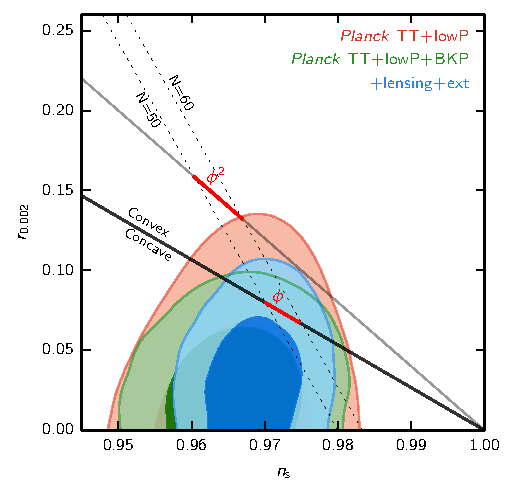
\includegraphics[keepaspectratio=true,scale=1.23]{ns_r_bicep}}}
\captionof{figure}{A contour plot of the likelihood functions for $r$ and $n_{s}$ taken from the 2015 Planck data release \cite{Planck}.}%      only if needed
\label{Fig3.1}
\end{minipage}

\newpage

\noindent%
\begin{minipage}{\linewidth}% to keep image and caption on one page
\makebox[\linewidth]{%        to center the image
  \fbox{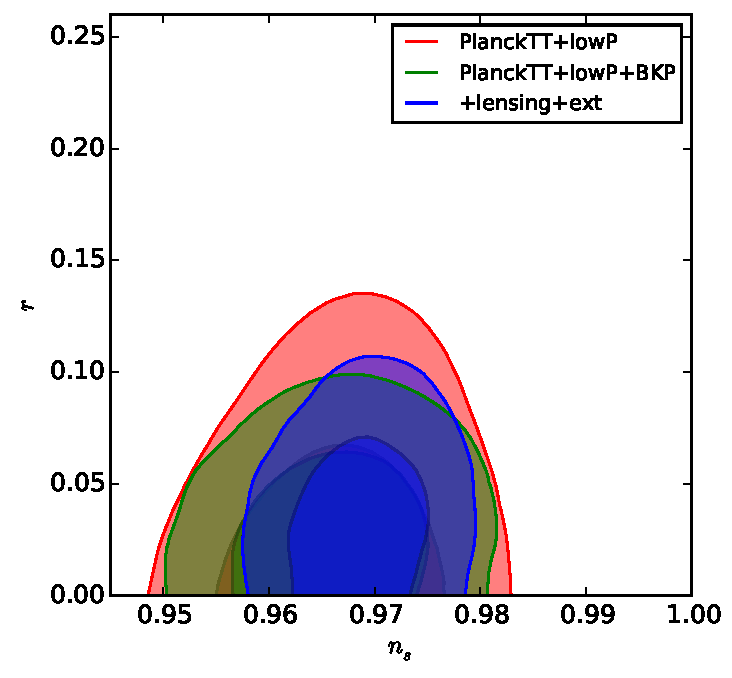
\includegraphics[keepaspectratio=true,scale=0.86]{ns_r_interp}}}
\captionof{figure}{Interpolated version of the likelihood functions for $r$ and $n_{s}$ taken from the 2015 Planck data release \cite{Planck}.}%      only if needed
\label{Fig3.2}
\end{minipage}

\subsection{Comparison with Slow-roll Predictions} \label{subsec:CompSloRoll}

As we should find our results differ from the slow-roll results because we are solving the Mukhanov equation whilst making no assumptions from slow-roll or for de-Sitter space, we should compare our results with the slow-roll predictions. These is done by plotting $r$ and $n_{s}$ with equations (\ref{eq2.86}), (\ref{eq2.87}) and (\ref{eq2.88}) along with our numerical solution where in particular we are interested in any differences from the second-order result for $n_{s}$ because that should agree with our data very closely. In our code, this is implemented by first setting the horizon crossing ($k = aH$) to be a desired number of e-folds before the end of inflation and then extracting the field value $\phi_{cross}$ and using that to compute $\epsilon$, $\eta$, $\xi$ and $\sigma$.

\section{Inflationary Potentials} \label{sec:InflatPots}

In order to test the differential equation solvers in our code, we pick several potentials to see how they compare with the observational constraints set out above.

\subsection{Chaotic Quadratic Potential} \label{subsec:ChaoSquPot}

The first potential we chose to test is the chaotic quadratic potential where:

\begin{equation} \label{eq3.37}
V(\phi) = \frac{1}{2} m^{2} \phi^{2},
\end{equation}

whose equation of motion given from equation (\ref{eq2.14}) in a flat space metric $\eta_{\mu\nu}$ is the Klein-Gordon equation. The scalar particle's mass $m$ is chosen to be $10^{-6}$ so the the COBE normalisation \cite{White:1995ic} of the anisotropies is satisfied. The quantities we need to compute $\phi^{\prime \prime}$ and $\phi^{\prime \prime \prime}$ that are needed to solve the perturbation equation are:

\begin{equation} \label{eq3.38}
\frac{V_{,\phi}(\phi)}{V(\phi)} = \frac{2}{\phi} \quad \mathrm{and} \quad \frac{d}{dN} \left( \frac{V_{,\phi}(\phi)}{V(\phi)} \right) = - \frac{2\phi^{\prime}}{\phi^{2}}.
\end{equation}

The slow-roll parameters for this potential are given by:

\begin{equation} \label{eq3.39}
\epsilon = \frac{2}{\phi^{2}} \quad , \quad \eta = \frac{2}{\phi^{2}} \quad , \quad \xi = 0 \quad , \quad \sigma =  0.
\end{equation}

\subsection{Chaotic Quartic Potential} \label{subsec:ChaoQuaPot}

The second potential is the chaotic quartic potential where:

\begin{equation}\label{eq3.40}
V(\phi) = \frac{1}{4} \lambda \phi^{4},
\end{equation}

where $\lambda$ is a constant given by $10^{-12}$ to fulfil the COBE normalisation in this case. This time the quantities needed to solve the perturbation equation are given by:

\begin{equation} \label{eq3.41}
\frac{V_{,\phi}(\phi)}{V(\phi)} = \frac{4}{\phi} \quad \mathrm{and} \quad \frac{d}{dN} \left( \frac{V_{,\phi}(\phi)}{V(\phi)} \right) = - \frac{4\phi^{\prime}}{\phi^{2}}.
\end{equation}

The slow-roll parameters for this potential are given by:

\begin{equation} \label{eq3.42}
\epsilon = \frac{8}{\phi^{2}} \quad , \quad \eta = \frac{12}{\phi^{2}} \quad , \quad \xi = \frac{96}{\phi^{4}} \quad , \quad \sigma = \frac{384}{\phi^{6}}
\end{equation}

\subsection{Axion Monodromy Potential} \label{subsec:AxoMonPot}

We also investigate a potential called `Axion Monodromy' that has motivations from string theory \cite{Silverstein:2008sg, Silverstein:2013wua} that is given by:

\begin{equation} \label{eq3.43}
V(\phi) = \lambda^{3} \phi,
\end{equation}

where this time the constant $\lambda$ is equal to $10^{-4}$ to satisfy the COBE normalisation. The quantities needed to solve the perturbation equation are:

\begin{equation} \label{eq3.44}
\frac{V_{,\phi}(\phi)}{V(\phi)} = \frac{1}{\phi} \quad \mathrm{and} \quad \frac{d}{dN} \left( \frac{V_{,\phi}(\phi)}{V(\phi)} \right) = - \frac{\phi^{\prime}}{\phi^{2}}.
\end{equation}

The slow-roll parameters for this potential are:

\begin{equation} \label{eq3.45}
\epsilon = \frac{1}{2\phi^{2}} \quad , \quad \eta = 0 \quad , \quad \xi = 0 \quad , \quad \sigma = 0.
\end{equation}


%-----------------------------------------------------
% Chapter: Results
%-----------------------------------------------------

\chapter{Results}
\label{chap:Results}

\section{Solutions of the Dynamics Equation} \label{sec:SolDynEq}

\subsection{Chaotic Quadratic Potential} \label{subsec:Res_Dyn_Square}

The solution for $\phi$ from equation (\ref{eq3.7}) is plotted below in figure \ref{Fig4.1}:

\noindent%
\begin{minipage}{\linewidth}% to keep image and caption on one page
\makebox[\linewidth]{%        to center the image
  \fbox{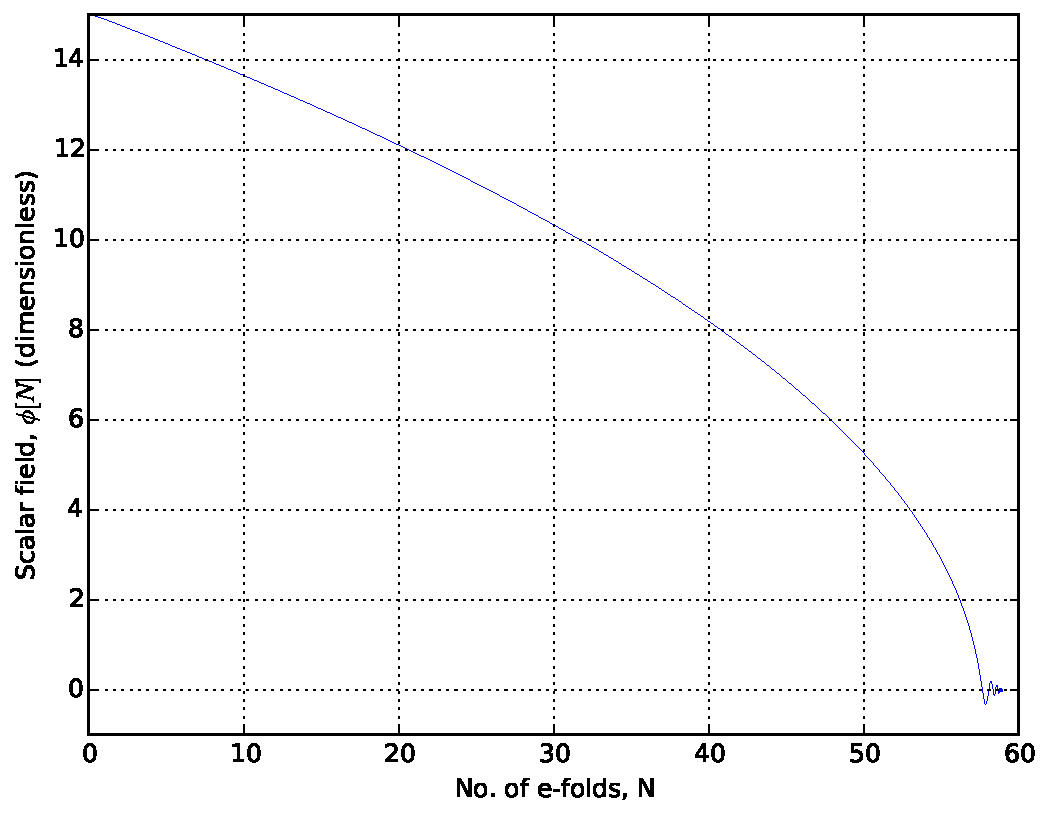
\includegraphics[keepaspectratio=true,scale=0.771]{square_PhiNPlt}}}
\captionof{figure}{A plot of the $\phi[N]$ solution given from the inflationary field dynamics equation for the potential $V = \frac{1}{2}m^{2}\phi^{2}$.}%      only if needed
\label{Fig4.1}
\end{minipage}
\\[10pt]

As we can see, initially the solution for $\phi[N]$ decays exponentially for approximately 56 e-folds before then oscillating around the minimum of the potential afterwards as mentioned in section \ref{subsec:ScalFieldsCurvST}. From this, we realise that inflation is lasting for the required 50-60 e-folds needed to solve the horizon and flatness problems which means the slow-roll predictions of $\phi_{0}$, $\phi_{end}$ and $N(\phi)$ described in section \ref{subsec:NoEfolds} are working well and that this potential obeys requirements of the slow-roll prediction very well. In order to study the end of inflation further, we provide the following plot of $\phi[N]$, $\epsilon$, $\eta$ and the inflation condition given in equation (\ref{eq3.25}) in figure \ref{Fig4.2} below.

\noindent%
\begin{minipage}{\linewidth}% to keep image and caption on one page
\makebox[\linewidth]{%        to center the image
  \fbox{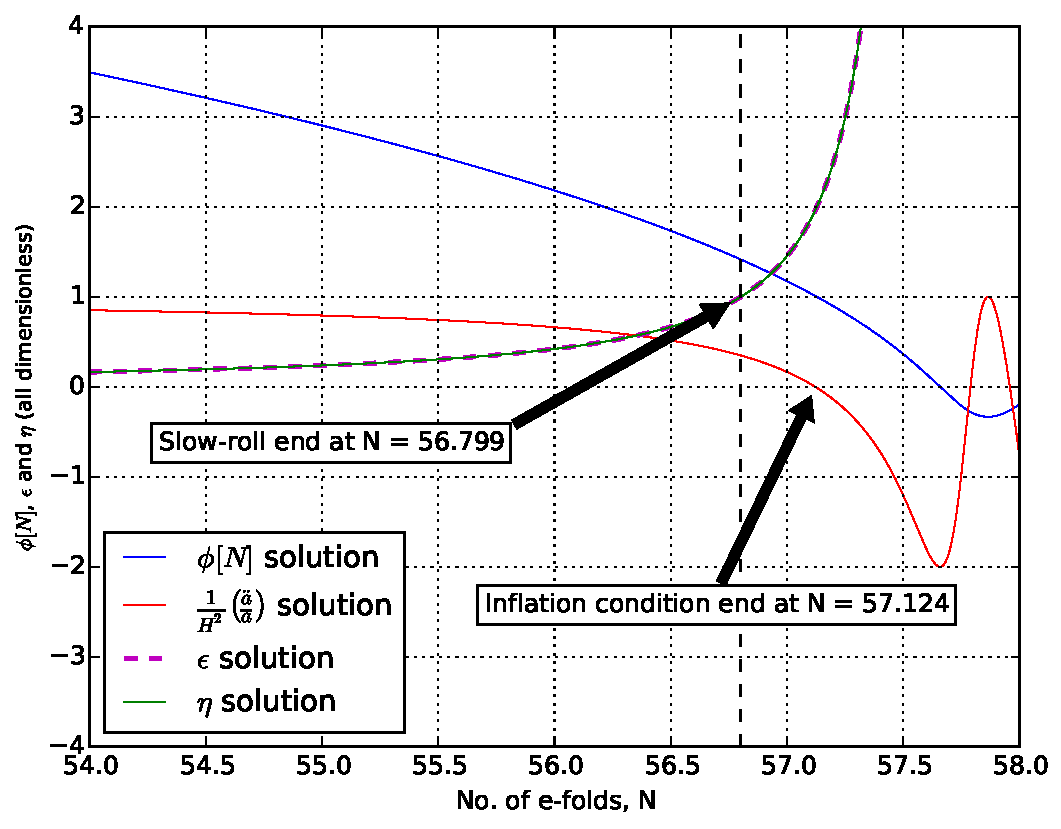
\includegraphics[keepaspectratio=true,scale=0.771]{square_CombinedNPlt}}}
\captionof{figure}{A plot of the $\phi[N]$ solution with the slow-roll parameters $\epsilon$ and $\eta$ and the inflationary condition at the end of inflation for the potential $V = \frac{1}{2}m^{2}\phi^{2}$.}%      only if needed
\label{Fig4.2}
\end{minipage}
\\[10pt]

As we can see, the $\phi[N]$ solution is just about to start oscillating in the 54 - 58 e-fold range here and that the inflationary condition also begins to oscillate in correspondence with the scalar field. The solutions for $\epsilon$ and $\eta$ however become asymptotic whenever the field and hence the potential are zero indicating that the slow-roll parameters are no longer useful after inflation as expected.

We also investigate two definitions for the end of inflation here with one being when $\ddot{a} = 0$ as seen in the inflationary condition and the other being when $\epsilon = 1$ (and $\eta$ for this potential). As we can see, there is a disparity between the two of approximately 0.3 e-folds between the actual condition and the slow-roll prediction. However as the slow-roll result is only different from the actual result by approximately 0.6\%, we think we are justified in using the slow-roll prediction later for the end of inflation in our perturbation equation solver but we will discuss this further in the discussion section.

Finally, we would also like to verify that the Hubble radius is becoming smaller with time as needed to satisfy inflationary condition (\ref{eq2.7}) and to solve the horizon problem. Therefore, we make the plot of equation (\ref{3.26}) for this potential with the result in figure \ref{Fig4.3} below.

\noindent%
\begin{minipage}{\linewidth}% to keep image and caption on one page
\makebox[\linewidth]{%        to center the image
  \fbox{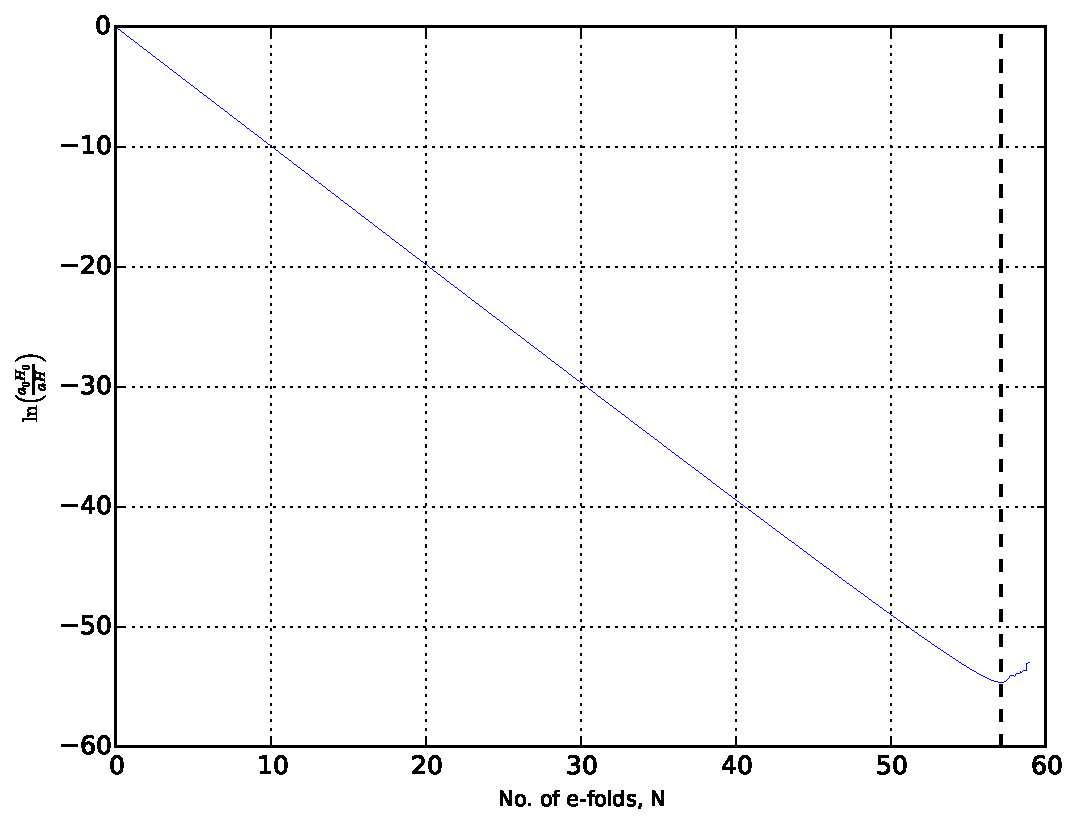
\includegraphics[keepaspectratio=true,scale=0.771]{square_HubbleRadiusInfCondition}}}
\captionof{figure}{A plot of the logarithm of the Hubble radius relative to the initial value of the Hubble radius against the number of e-folds $N$ for the quadratic potential.}%      only if needed
\label{Fig4.3}
\end{minipage}
\\[10pt]

As we can see from the plot above, throughout inflation the Hubble radius is monotonically decreasing where the slow-roll prediction of the end of inflation is indicated by the vertical dashed line. We also note that the logarithm yields a straight line as expected for the log of the exponential $e^{Ht}$ in addition to verifying that $H \sim \mathrm{const.}$ throughout inflation as the gradient of this line changes very little throughout. After inflation is finished, we notice that the gradient becomes positive as expected which indicates scales can now begin to re-enter the horizon.

\subsection{Chaotic Quartic Potential} \label{subsec:Res_Dyn_Quartic}

As can be seen in figure \ref{Fig4.4} below, we also make a plot of $\phi[N]$ for the quartic potential where as we can see the field is larger in magnitude which is due to the larger power in the potential term. This time we see that this potential yields approximately 50 e-folds of inflation where the field is decaying exponentially before becoming oscillatory about the minimum of the potential.

As before, we use \ref{Fig4.5} below to investigate the end of inflation for this potential where we again see the oscillatory behaviour of the solution for $\phi[N]$ and the inflation condition and as well as observing the slow-roll parameters again. This time the disparity between the end of inflation measurements is approximately 0.4 e-folds which is within 0.7\% of the true value given from the inflation condition which further verifies the validity of the slow-roll approximation.

\noindent%
\begin{minipage}{\linewidth}% to keep image and caption on one page
\makebox[\linewidth]{%        to center the image
  \fbox{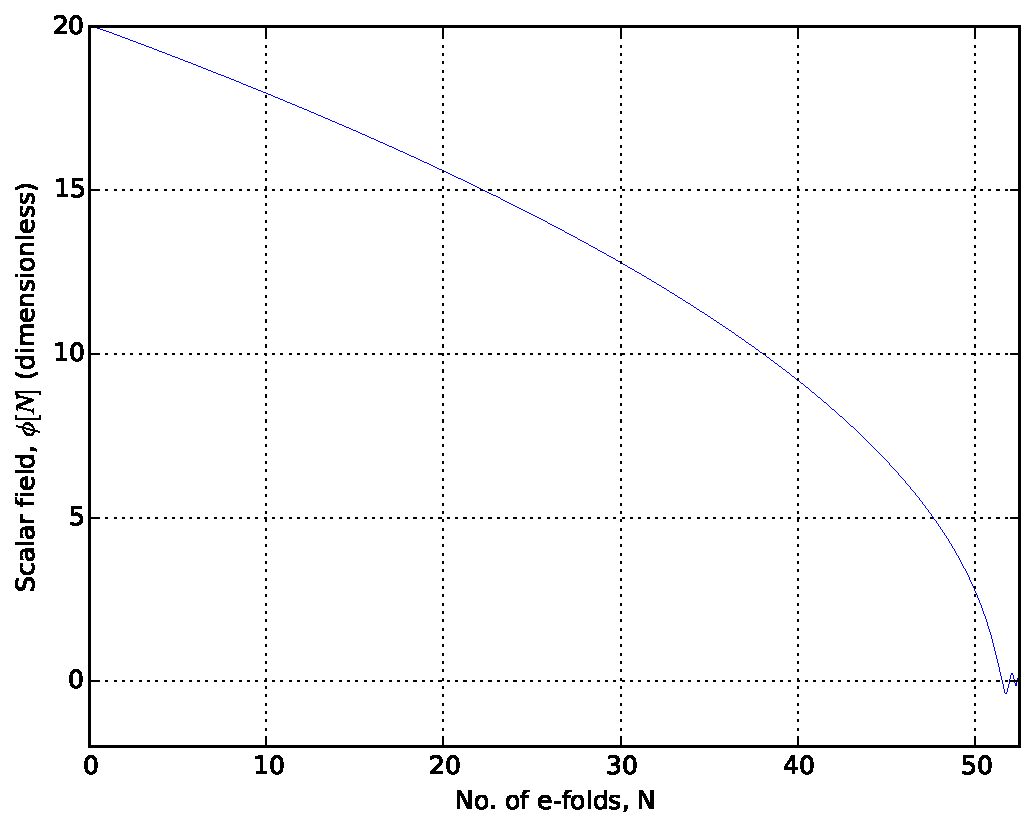
\includegraphics[keepaspectratio=true,scale=0.771]{quartic_PhiNPlt}}}
\captionof{figure}{A plot of the $\phi[N]$ solution given from the inflationary field dynamics equation for the potential $V = \frac{1}{4}\lambda \phi^{4}$.}%      only if needed
\label{Fig4.4}
\end{minipage}

\noindent%
\begin{minipage}{\linewidth}% to keep image and caption on one page
\makebox[\linewidth]{%        to center the image
  \fbox{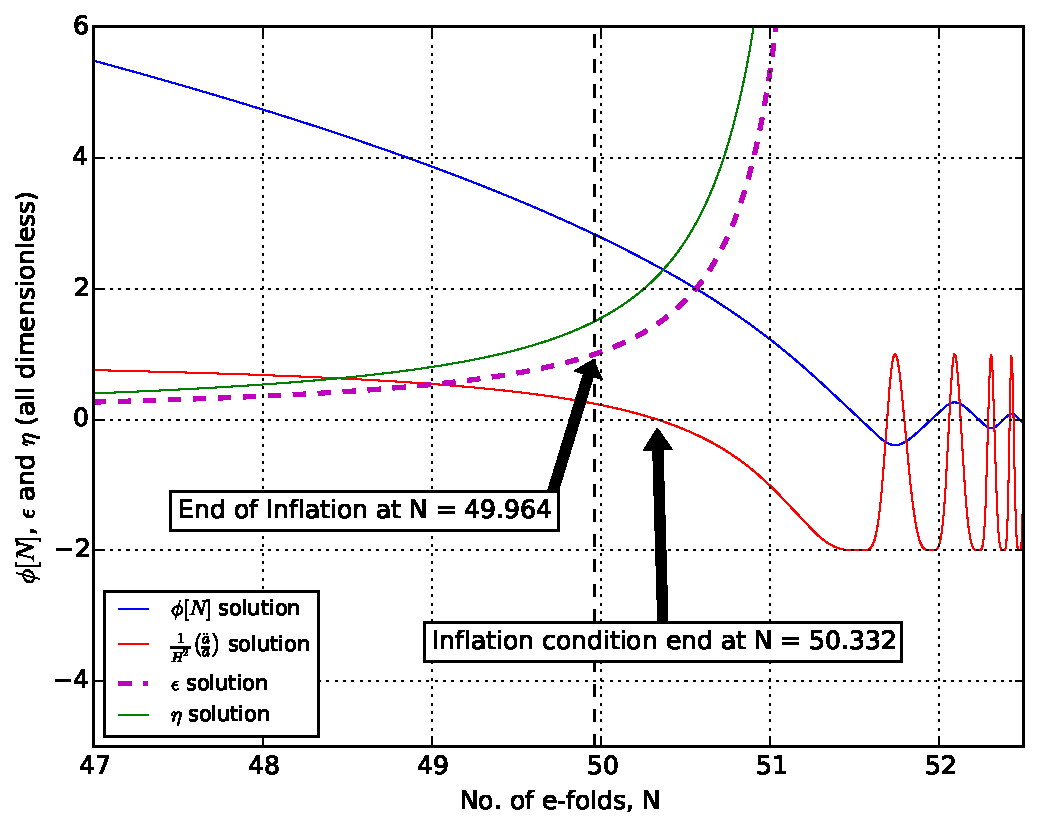
\includegraphics[keepaspectratio=true,scale=0.771]{quartic_CombinedNPlt}}}
\captionof{figure}{A plot of the $\phi[N]$ solution with the slow-roll parameters $\epsilon$ and $\eta$ and the inflationary condition at the end of inflation for the potential $V = \frac{1}{4}\lambda\phi^{4}$.}%      only if needed
\label{Fig4.5}
\end{minipage}

From figure \ref{Fig4.6} below, we again observe the expected negative gradient straight line behaviour of the logarithm of the Hubble radius throughout inflation before then starting to increase after inflation has finished. We also note that the divergences in the plot after inflation are caused by Python not having the resolution to track the $\phi$ dependence of the Hubble parameter during the rapid field oscillation epoch.

\noindent%
\begin{minipage}{\linewidth}% to keep image and caption on one page
\makebox[\linewidth]{%        to center the image
  \fbox{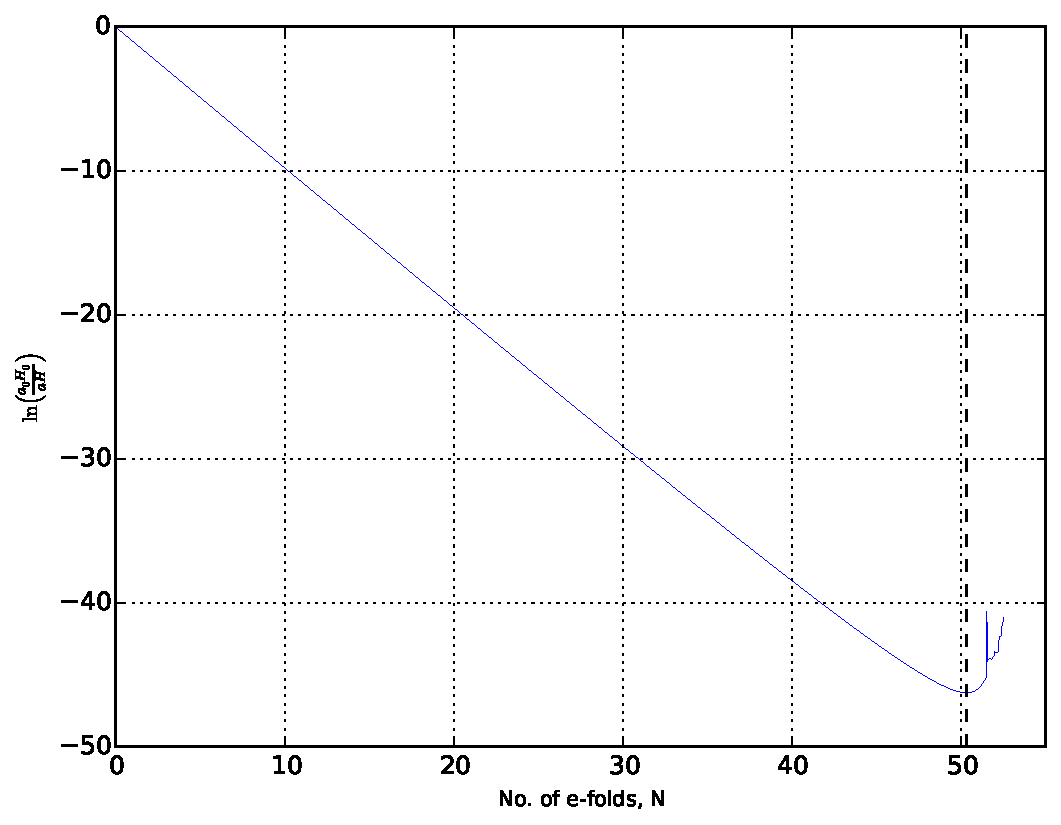
\includegraphics[keepaspectratio=true,scale=0.771]{quartic_HubbleRadiusInfCondition}}}
\captionof{figure}{A plot of the logarithm of the Hubble radius relative to the initial value of the Hubble radius against the number of e-folds $N$ for the quartic potential.}%      only if needed
\label{Fig4.6}
\end{minipage}
\\[10pt]

\subsection{Axion Monodromy Potential} \label{subsec:Res_Dyn_Quartic}

As can be seen in figure \ref{Fig4.7} below, we also make a plot of $\phi[N]$ for the axion monodromy potential which does not exhibit the oscillations after inflation has finished because the linear potential has no minimum to oscillate around. This can be seen in \ref{Fig4.8} where the Hubble parameter $H$ has become infinitesimally small and the $H^{-2}$ dependence in the dynamics equation (\ref{eq3.7}) has caused the inflation field solution to diverge. However, we are interested in solving the perturbation equations during inflation so therefore we ensure that perturbations are not evaluated after inflation has finished.

We can see this divergence in greater detail in figure \ref{Fig4.8} where the epoch of the end of inflation is found for this potential. This time the disparity between the two predictions for the end of inflation is approximately 0.3 e-folds with a relative error of 0.5\%.

Finally, we also verify that the comoving Hubble radius is decreasing in size with this potential in figure \ref{Fig4.9} where as before we see this happens at a constant rate until the end of inflation where it begins to increase in size. However in this case, the increase is mainly caused by the divergence of $H$ after inflation.

\noindent%
\begin{minipage}{\linewidth}% to keep image and caption on one page
\makebox[\linewidth]{%        to center the image
  \fbox{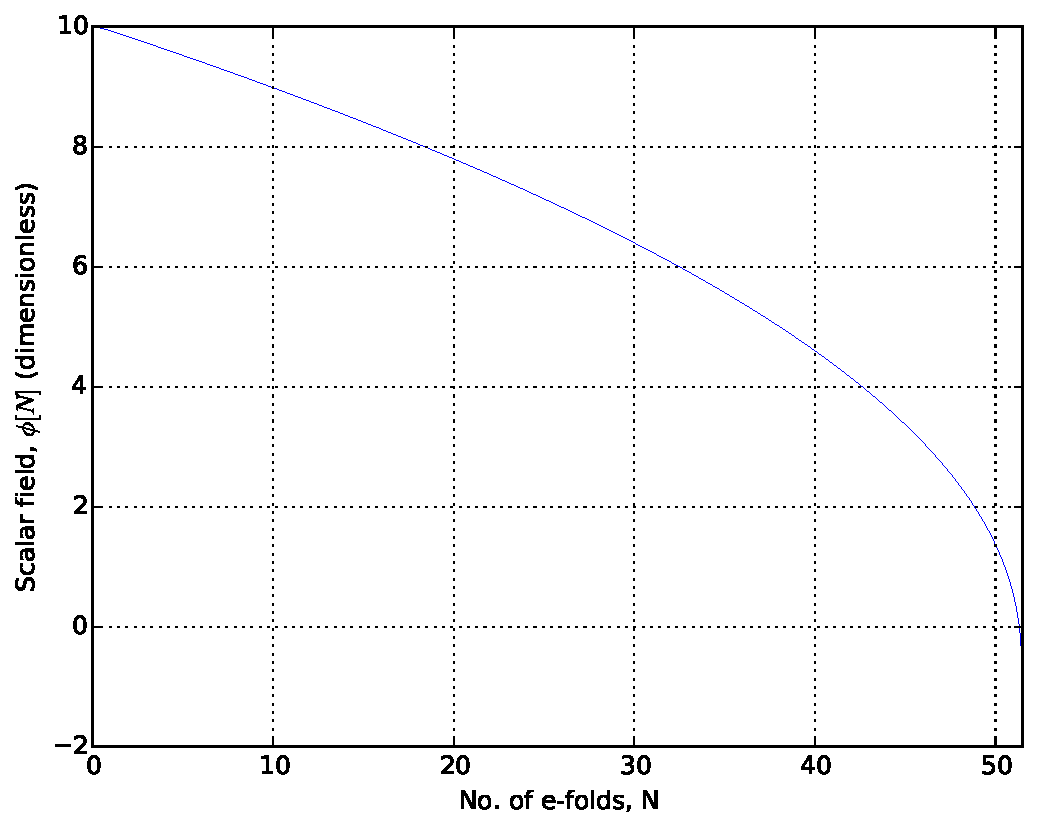
\includegraphics[keepaspectratio=true,scale=0.771]{mono_PhiNPlt}}}
\captionof{figure}{A plot of the $\phi[N]$ solution given from the inflationary field dynamics equation for the potential $V = \lambda^{3} \phi$.}%      only if needed
\label{Fig4.7}
\end{minipage}

\noindent%
\begin{minipage}{\linewidth}% to keep image and caption on one page
\makebox[\linewidth]{%        to center the image
  \fbox{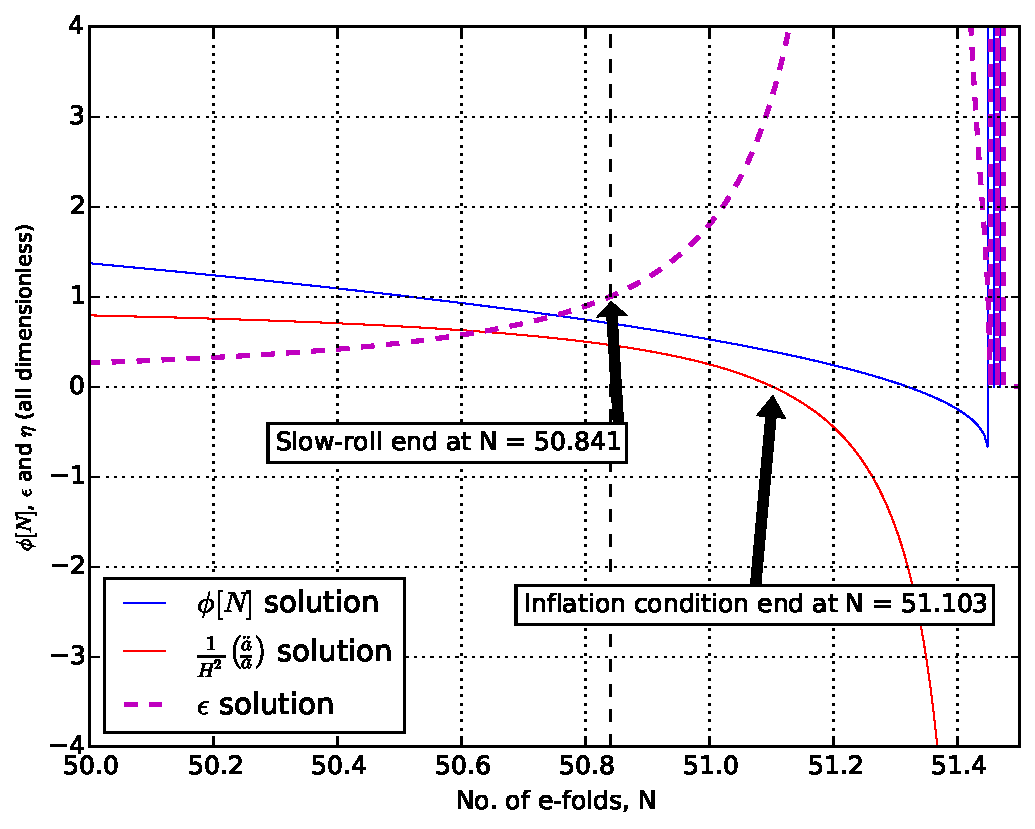
\includegraphics[keepaspectratio=true,scale=0.771]{mono_CombinedNPlt}}}
\captionof{figure}{A plot of the $\phi[N]$ solution with the slow-roll parameters $\epsilon$ and $\eta$ and the inflationary condition at the end of inflation for the potential $V = \lambda^{3}\phi$.}%      only if needed
\label{Fig4.8}
\end{minipage}

\noindent%
\begin{minipage}{\linewidth}% to keep image and caption on one page
\makebox[\linewidth]{%        to center the image
  \fbox{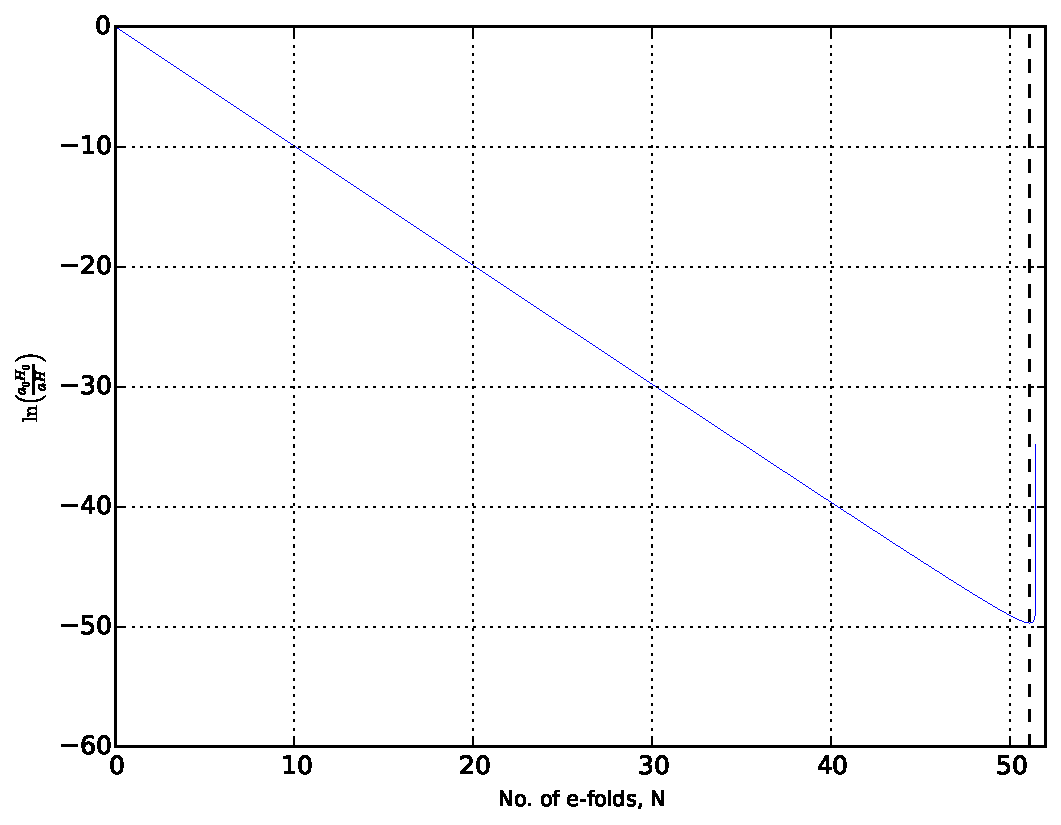
\includegraphics[keepaspectratio=true,scale=0.771]{mono_HubbleRadiusInfCondition}}}
\captionof{figure}{A plot of the logarithm of the Hubble radius relative to the initial value of the Hubble radius against the number of e-folds $N$ for the axion monodromy potential.}%      only if needed
\label{Fig4.9}
\end{minipage}

\section{Solutions of the Perturbation Equations} \label{sec:SolPertEquat}

\subsection{Chaotic Quadratic Potential} \label{subsec:Res_Pert_Square}

As mentioned in section \ref{subsec:InitCondKmod}, we integrated the real and imaginary parts of the perturbation equation separately and then used the results from section \ref{subsec:CalcPowSpec} to find the scalar and tensor power spectra as can be seen in figures \ref{Fig4.10} and \ref{Fig4.11} below. In these graphs, the wave-mode $k$ values are given in the legend where the smallest corresponds with 60 e-folds and the largest corresponds with 50 e-folds before the end of inflation. These horizon crossing points can be seen at the turning points of the spectra where each converges to a near constant value afterwards. We also note that smaller wave-modes (or an earlier horizon crossing point) gives the largest spectrum where each successively larger wave-mode then gives a smaller spectra each time. This behaviour is supposed to lead to initial inhomogeneities in the universe which then evolves to become the large-scale structure we see today. If we look at the values of the scalar and tensor spectra at our chosen value of 45 e-folds, we see that the tensor values are approximately an order of magnitude smaller than the scalars so we should expect the tensor to scalar ratio $r$ to be $\mathcal{O}(10^{-1})$.

In section \ref{subsec:ScalSpecIndex}, we discussed using a quadratic fit on the $\ln(k)$ vs. $\ln(\Delta_{s}^{2})$ curve to obtain the spectral index where we can see the results in figure \ref{Fig4.12} below. As we can see, the quadratic fit is an excellent fit to our data with almost no quadratic dependence at all and therefore justifies calculating the spectral index with this method. As all of our tested potentials were as successful as this one, we only include this one as a demonstration.

\noindent%
\begin{minipage}{\linewidth}% to keep image and caption on one page
\makebox[\linewidth]{%        to center the image
  \fbox{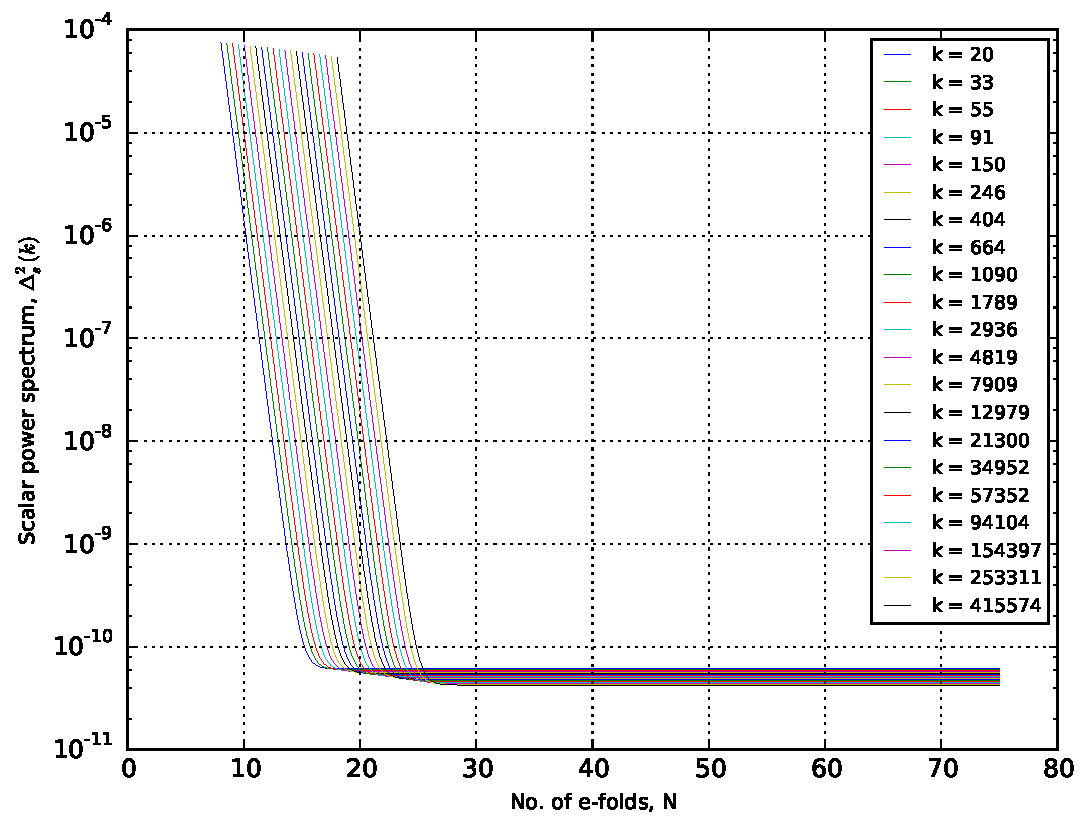
\includegraphics[keepaspectratio=true,scale=0.771]{Square_AllScalarPerts}}}
\captionof{figure}{A plot of the scalar power time dependance for k values corresponding with horizon crossing between 50 and 60 e-folds before the end of inflation for $V = \frac{1}{2}m^{2}\phi^{2}$.}%      only if needed
\label{Fig4.10}
\end{minipage}

\noindent%
\begin{minipage}{\linewidth}% to keep image and caption on one page
\makebox[\linewidth]{%        to center the image
  \fbox{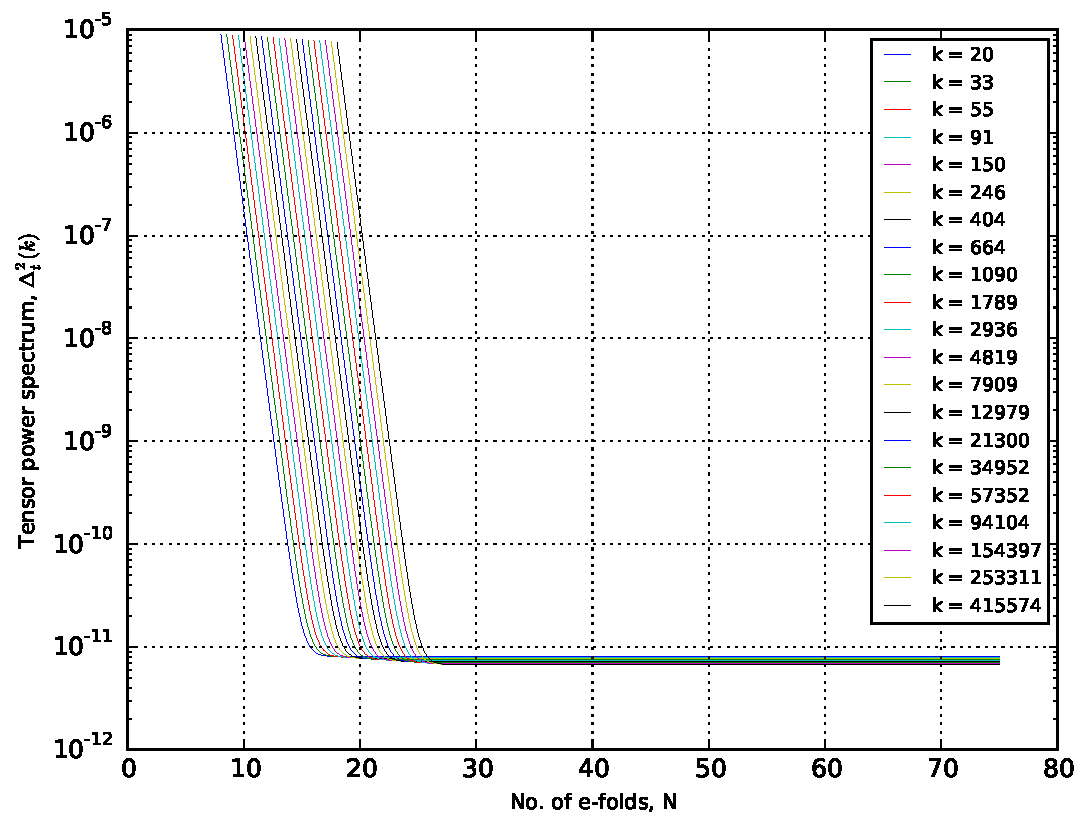
\includegraphics[keepaspectratio=true,scale=0.771]{Square_AllTensorPerts}}}
\captionof{figure}{A plot of the tensor power time dependance for k values corresponding with horizon crossing between 50 and 60 e-folds before the end of inflation for $V = \frac{1}{2}m^{2}\phi^{2}$}%      only if needed
\label{Fig4.11}
\end{minipage}

\noindent%
\begin{minipage}{\linewidth}% to keep image and caption on one page
\makebox[\linewidth]{%        to center the image
  \fbox{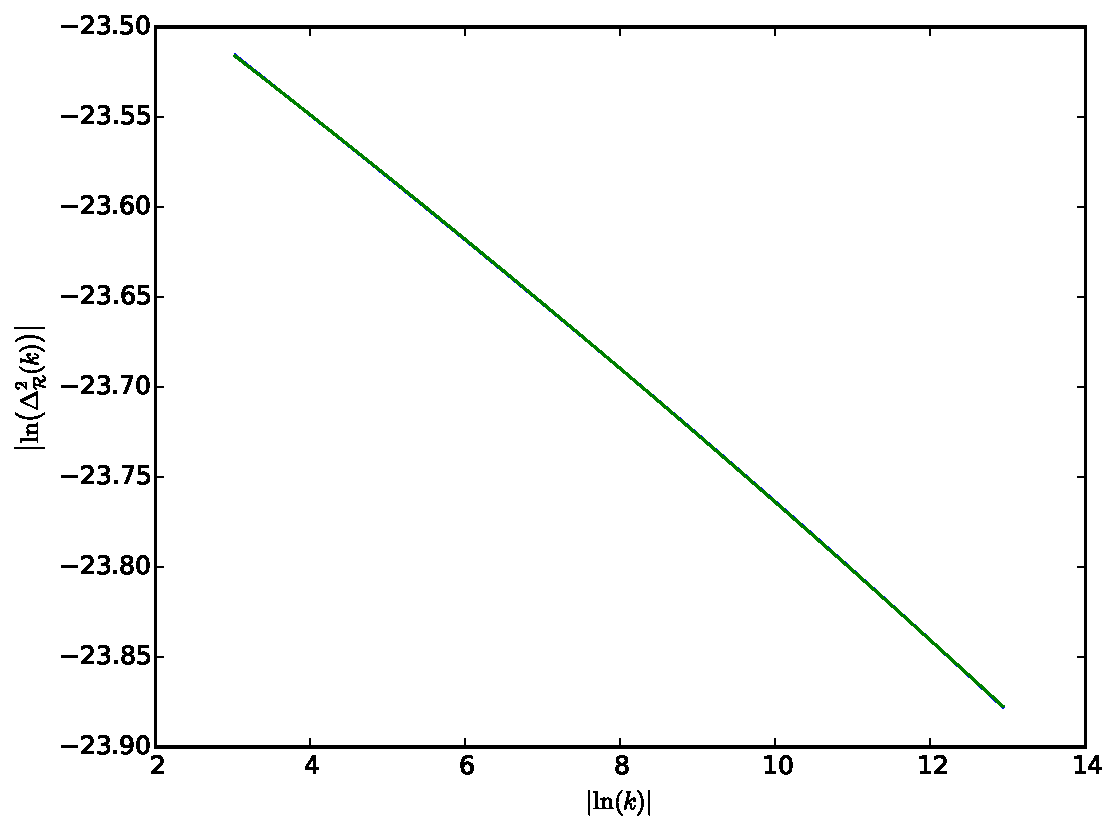
\includegraphics[keepaspectratio=true,scale=0.6]{Square_ScalSpecKplt}}}
\captionof{figure}{A plot of the quadratic fit used to find the scalar spectral indices for the quadratic potential.}%      only if needed
\label{Fig4.12}
\end{minipage}

Next we computed the tensor to scalar ratio and scalar spectral indices exactly and plotted the results as seen in figure \ref{Fig4.13} below. 

\noindent%
\begin{minipage}{\linewidth}% to keep image and caption on one page
\makebox[\linewidth]{%        to center the image
  \fbox{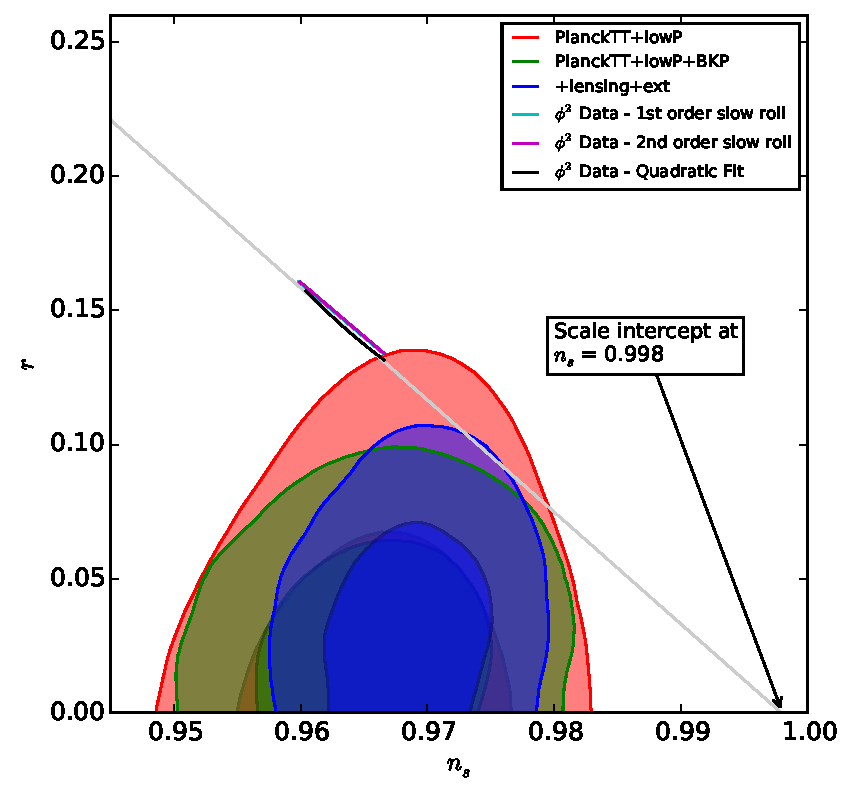
\includegraphics[keepaspectratio=true,scale=0.85]{Square_ns_r}}}
\captionof{figure}{A plot of the scalar spectral indices against the tensor to scalar ratios for the quadratic potential with the contour data provided from the 2015 Planck release \cite{Planck}.}%      only if needed
\label{Fig4.12}
\end{minipage} \\[10pt]

As predicted, we find the tensor to scalar ratio to be 0.16 for horizon crossing at 50 e-folds before the end of inflation and 0.13 for horizon crossing at 60 e-folds before the end of inflation. We also observe a range of 0.961 - 0.968 for the scalar spectral indices over the same range of horizon crossing points. As we can see, this is in strong agreement with both the first and second order slow rollpredictions for this potential. However as both of these parameter  are well outside of the 2-sigma limits of the Planck data, we have to conclude that the chaotic quadratic potential is very unlikely to be a candidate for the inflationary potential.Also as a means of providing another consistency check for our integrator, we fit a straight line to our data and calculated the point where it crosses the $n_{s}$ axis where it should be unity because scale invariance would imply the tensor to scalar ratio was zero. Here we find it crosses at 0.998 which is within 0.2\% of unity and further confirms that we are evaluating the perturbations correctly.

\subsection{Chaotic Quartic Potential} \label{subsec:Res_Pert_Quart}

Next, we investigated the chaotic quartic potential where we can see the scalar and tensor power spectra plotted again in figures \ref{Fig4.14} and \ref{Fig4.15} below. The first thing we notice is that the range of $k$ values (456 - 8403488) for this potential are a lot higher than the values in the quadratic potential case. This is because when we set $k = aH$ for horizon crossing, the potential dependance in the Hubble parameter causes it to be much larger. Once again, we see that the power spectra become smaller for increasing $k$ values and increasing number of e-folds before the end of inflation. At 45 e-folds, we notice that the scalar power spectra are approximately three times larger than the tensor power spectra so that we should expect the tensor to scalar ratio to be $\sim 0.3$ for each k-mode.

\noindent%
\begin{minipage}{\linewidth}% to keep image and caption on one page
\makebox[\linewidth]{%        to center the image
  \fbox{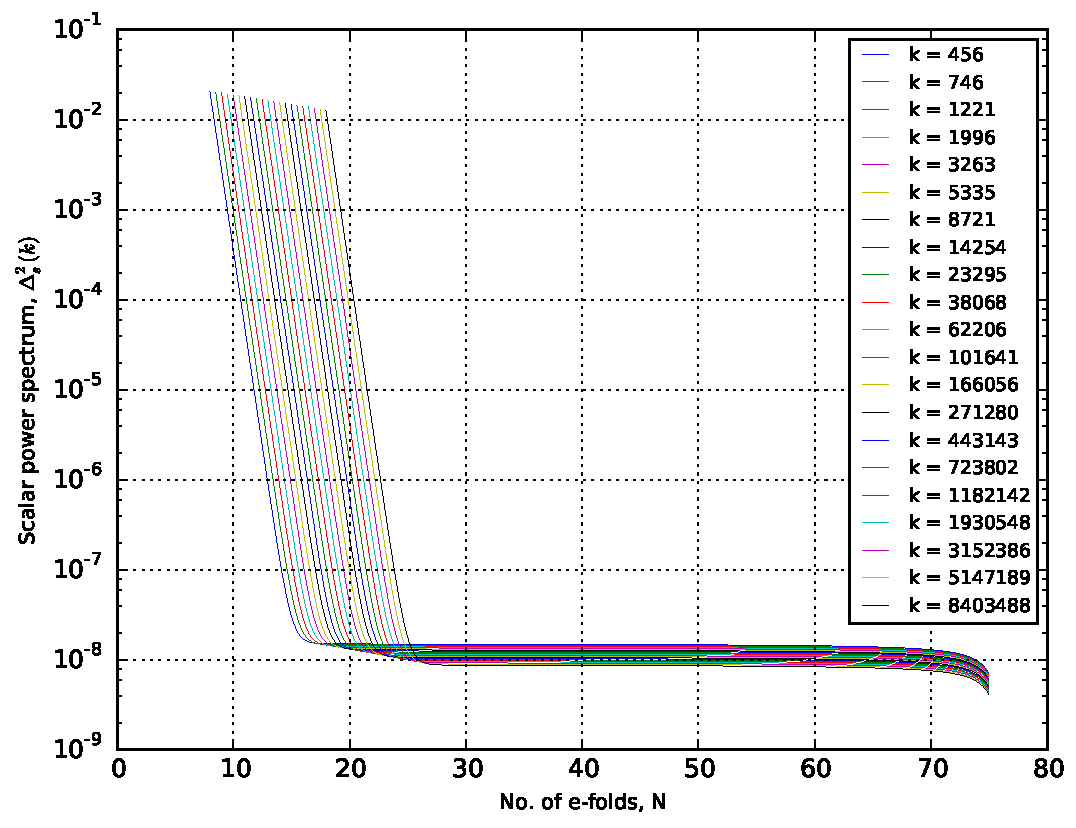
\includegraphics[keepaspectratio=true,scale=0.771]{Quartic_AllScalarPerts}}}
\captionof{figure}{A plot of the scalar power time dependance for k values corresponding with horizon crossing between 50 and 60 e-folds before the end of inflation for $V = \frac{1}{4}\lambda\phi^{4}.$}%      only if needed
\label{Fig4.14}
\end{minipage}

\noindent%
\begin{minipage}{\linewidth}% to keep image and caption on one page
\makebox[\linewidth]{%        to center the image
  \fbox{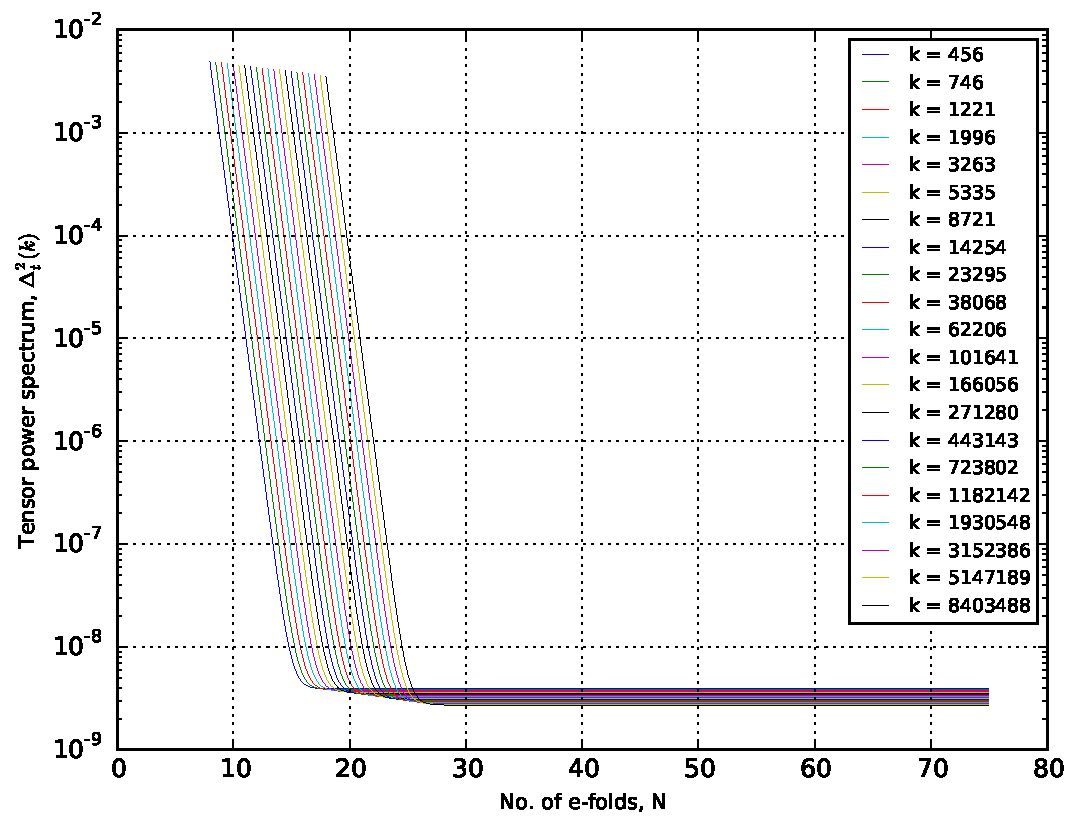
\includegraphics[keepaspectratio=true,scale=0.771]{Quartic_AllTensorPerts}}}
\captionof{figure}{A plot of the tensor power time dependance for k values corresponding with horizon crossing between 50 and 60 e-folds before the end of inflation for $V = \frac{1}{4}\lambda\phi^{4}$.}%      only if needed
\label{Fig4.15}
\end{minipage}

\noindent%
\begin{minipage}{\linewidth}% to keep image and caption on one page
\makebox[\linewidth]{%        to center the image
  \fbox{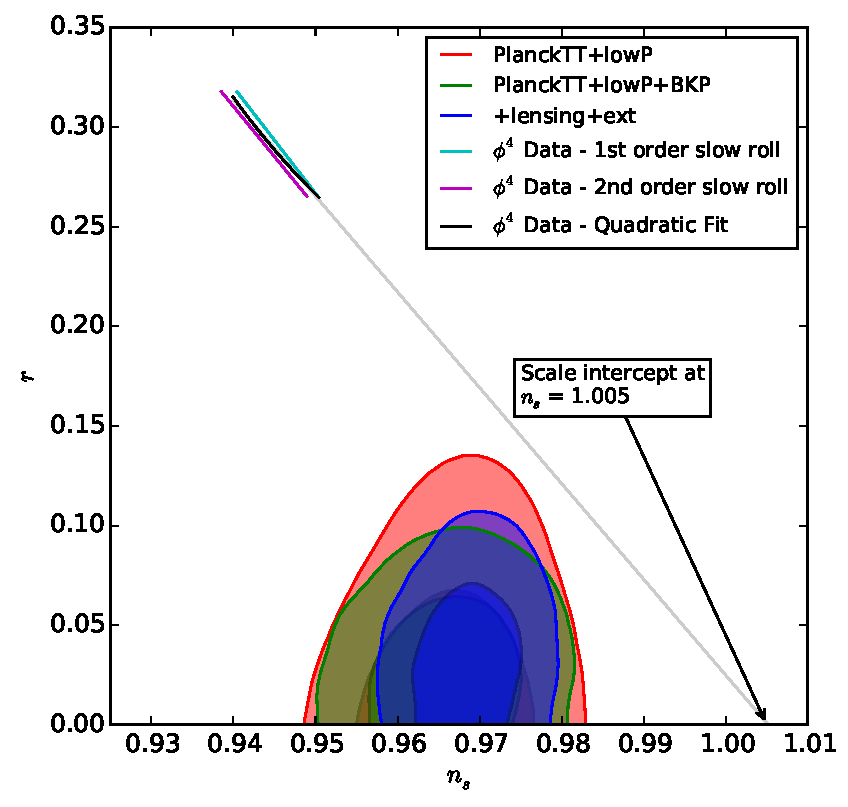
\includegraphics[keepaspectratio=true,scale=0.794]{Quartic_ns_r}}}
\captionof{figure}{A plot of the scalar spectral indices against the tensor to scalar ratios for the quartic potential with the contour data provided from the 2015 Planck release \cite{Planck}.}%      only if needed
\label{Fig4.16}
\end{minipage}

We therefore computed the tensor to scalar ratios and scalar spectral indices for this potential and plotted the results in figure \ref{Fig4.16} above. This time we find the tensor to scalar ratio to be 0.32 for a scale that crosses the horizon 50 e-folds before the end of inflation and 0.27 for a scale that crosses the horizon at 60 e-folds before the end of inflation. The range of scalar spectral indices that correspond with this is 0.94 and 0.95 for 50 and 60 e-folds before the end of inflation respectively. These results are very far from the largest constraint set out by Planck so that the quartic potential is not a candidate for inflation in our universe without modification. 

The results sit in between the first and second order slow roll results with the same shape so again we see that our integrator is consistent with other means of calculations. In addition to this, we see that our results show that we have scale invariance at $n_{s} = 1.005$ which is within 0.5\% of the expected value of 1 which is a further confirmation of our result's validity.

\subsection{Axion Monodromy Potential} \label{subsec:Res_Pert_Axion}

The last potential to be investigated was the axion monodromy potential where we can see the results for the scalar and tensor power spectra in figures \ref{Fig4.17} and \ref{Fig4.18} below. This potential has much smaller values for a given field value $\phi$ so in turn we have much smaller wave-modes ($6 \le k \le 131235$) needed for horizon crossing and therefore smaller power spectra values than the other two potentials. At $N = 45$, we see that the scalar power spectra values are more than a order of magnitude larger than the tensor power spectra so we should expect the tensor to scalar ratio to be $\le 0.1$. Also the spectra values here are closer together than the other two potentials so we should see $n_{s}$ closer to one.

\noindent%
\begin{minipage}{\linewidth}% to keep image and caption on one page
\makebox[\linewidth]{%        to center the image
  \fbox{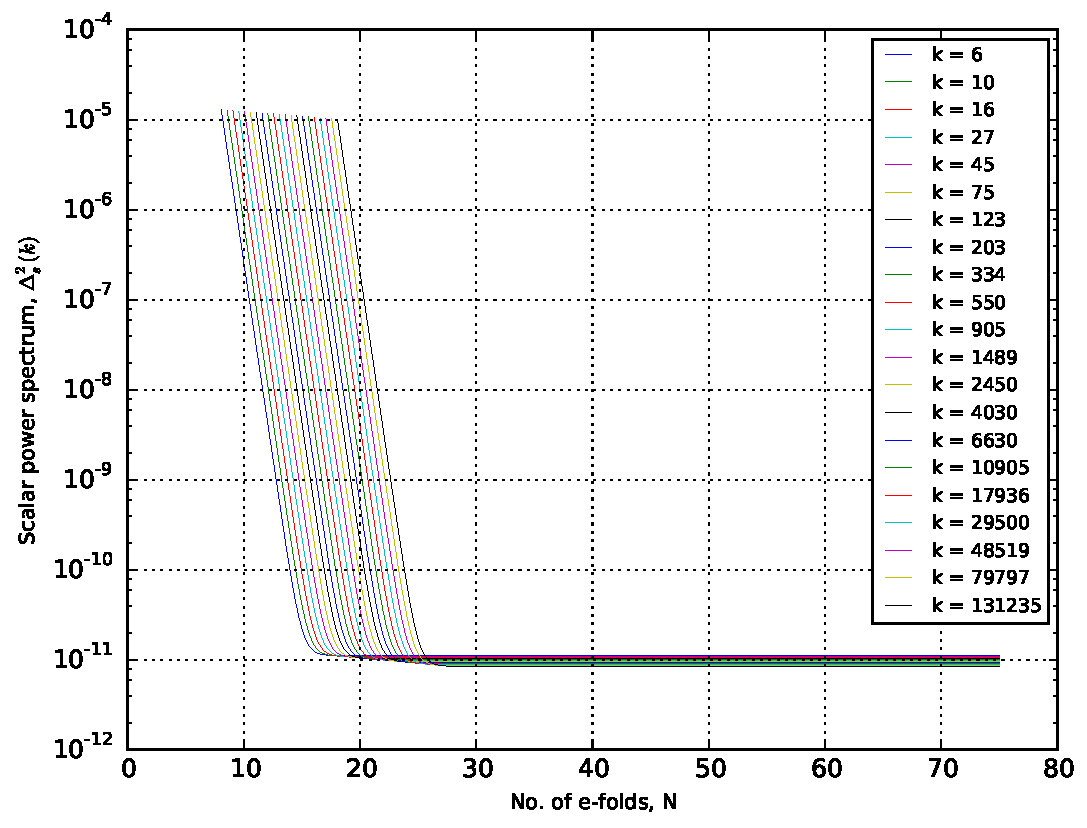
\includegraphics[keepaspectratio=true,scale=0.771]{Axion_AllScalarPerts}}}
\captionof{figure}{A plot of the scalar power time dependance for k values corresponding with horizon crossing between 50 and 60 e-folds before the end of inflation for $V = \lambda\phi$.}%      only if needed
\label{Fig4.17}
\end{minipage}

\noindent%
\begin{minipage}{\linewidth}% to keep image and caption on one page
\makebox[\linewidth]{%        to center the image
  \fbox{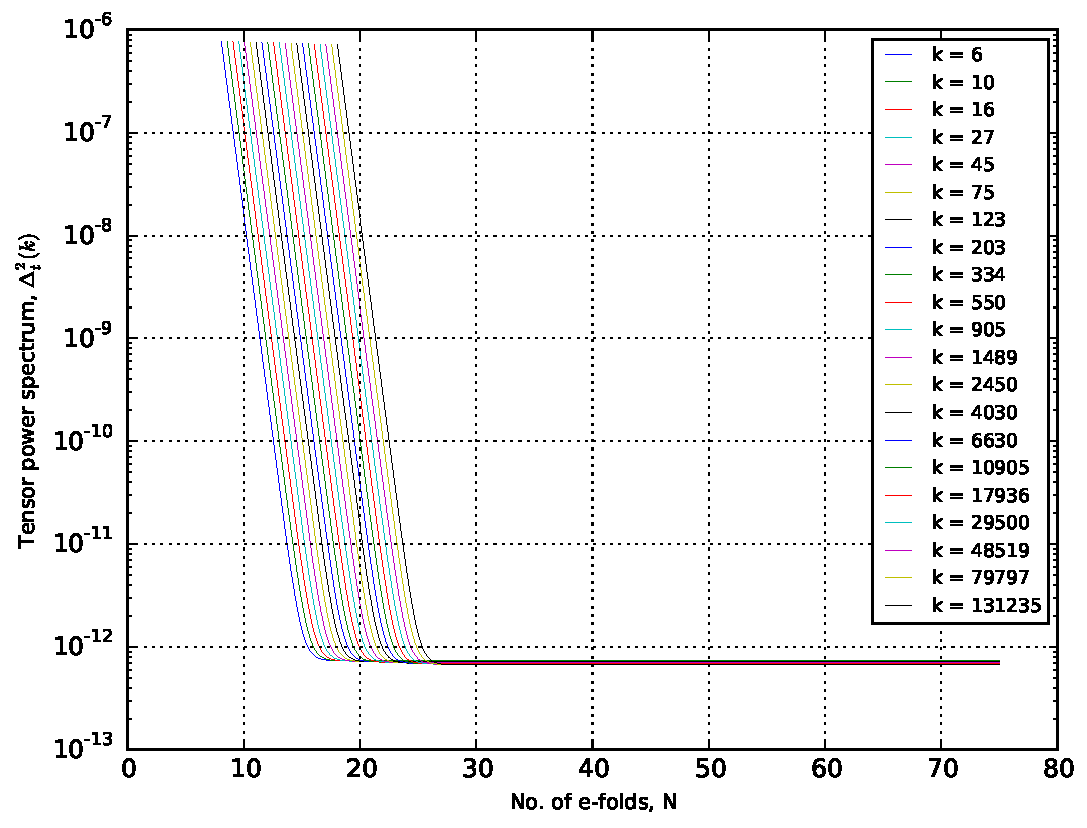
\includegraphics[keepaspectratio=true,scale=0.771]{Axion_AllTensorPerts}}}
\captionof{figure}{A plot of the tensor power time dependance for k values corresponding with horizon crossing between 50 and 60 e-folds before the end of inflation for $V = \lambda\phi$.}%      only if needed
\label{Fig4.18}
\end{minipage}

\noindent%
\begin{minipage}{\linewidth}% to keep image and caption on one page
\makebox[\linewidth]{%        to center the image
  \fbox{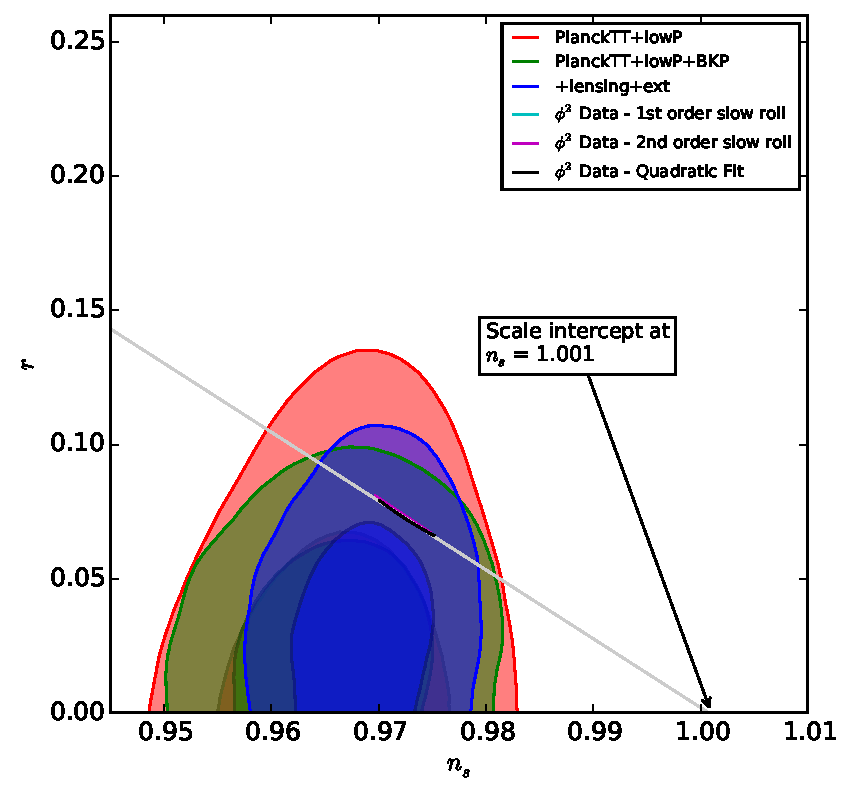
\includegraphics[keepaspectratio=true,scale=0.794]{Axion_ns_r}}}
\captionof{figure}{A plot of the scalar spectral indices against the tensor to scalar ratios for the axion  potential with the contour data provided from the 2015 Planck release \cite{Planck}.}%      only if needed
\label{Fig4.19}
\end{minipage}

The exact results for the tensor to scalar ratios and scalar spectral indices for each wave-mode are plotted in figure \ref{Fig4.19} above. This time we see the tensor to scalar ratio is 0.08 for a scale that crosses the horizon 50 e-folds before the end of inflation and is 0.06 for a scale that crosses the horizon 60 e-folds before the end of inflation. The corresponding scalar spectral indices are 0.97 and 0.975 for 50 and 60 e-folds before the end of inflation respectively. These results are well within the 2$\sigma$ bounds set by every type of measurement made by Planck so the axion monodromy potential is still a candidate for generating inflation. However the axion results do not sit within the 1$\sigma$ bound and it will be a long time before more precise measurements of the B-modes in the CMB are made by BICEP3 and other telescopes around 2016.

These results are almost exactly the same as the first and second slow roll predictions again here and also we see that the scalar spectral index value when the ratio is zero is 1.001 or within 0.1\% of the expected value and therefore we confirm these result's validity with other means of calculation.


%-----------------------------------------------------
% Chapter: Discussion
%-----------------------------------------------------

\chapter{Discussion}
\label{chap:Discuss}

We have successfully built a program that can solve the Mukhanov-Sasaki equation in full detail and produce scalar and tensor power spectra with their observables without using the slow-roll approximation and has the capacity to be applied to more complicated inflationary potentials such as multi-field or non-minimally coupled examples. This has been shown by the code's ability to reproduce existing results for well tested potentials to within a high degree of accuracy for each case. In addition to this, we have also demonstrated that some potentials are incompatible with observational data from Planck without major modification.

When solving the inflation field dynamics equation, we found the solution to be the expected exponential decay as a function of time (e-folds, N) during inflation before becoming a damped harmonic oscillator solution after inflation for two of the three tested potentials. The exception here was the axion monodromy potential which is an example of a small-field potential where lack of a minimum in the potential and the small field caused the solution for the Hubble parameter to diverge shortly after inflation had finished. This caused there to be numerical problems in our solution due to Python's variable resolution and therefore we must conclude our program is valid only throughout the duration of inflation. However, we did find an estimation of the end of inflation from the slow-roll approximation to be the same as the one from the inflationary condition to within 0.6\% for the three potentials. While 0.6\% is very low, we find the difference between the exact numerical solution and the slow-roll solution results for the power spectra to be much less than this so this difference is not negligible and should be corrected in a future study. Finally, we also verified that the inflation conditions discussed in section \ref{sec:CondInflation} are satisfied where we found that each tested potential did uphold these but only during inflation. In order to study the universe beyond inflation, it is clear that a consistent theory of reheating would be needed to properly describe the physics involved. However, as we only needed the results from the dynamics equation during inflation, this is not an issue for the solving the perturbation equations.

When progressing on to solving the perturbation equations, we found the expected near-constant power spectra after horizon crossing for each wave-mode corresponding with horizon crossing between 50 and 60 e-folds before inflation finishes. Before horizon crossing, the real and imaginary modes each have harmonic oscillator solutions that decay with increasing time that combine proportional to $\tau^{-1}$ as given by equation (\ref{eq2.73}). When studying the two quadratic and quartic power law inflation models, we found they both sit outside of the 95\% confidence region as predicted by the 2013 Planck data \cite{Planck:2013jfk}. However the axion monodromy potential results lie well within these limits as expected from \cite{Burgess:2013sla} and therefore we conclude our integrator is consistent with other methods used for calculating inflation's observables. In addition to this, our code gave similar results to the first- and second-order slow-roll results whilst being visibly different as well as always giving scale invariance at $n_{s} = 1$ to within $\sim$0.3\% for each of our potentials. These further tests indicate our program is suitable for computing higher order corrections needed to analyse potentials that do not obey the slow-roll conditions. Despite the agreement with the slow-roll results, the second-order slow-roll estimations were not any better than the first order results in comparison with our exact result for any of the potentials. This indicates that departure from slow-roll can be significant and should be accounted for in future studies.


%-----------------------------------------------------
% Chapter: Conclusions
%-----------------------------------------------------

\chapter{Conclusions}
\label{chap:Conclusions}

Having reviewed existing basic cosmological models and their problems, we have established the inflationary paradigm generated by a scalar field subject to a very particular set of conditions to give the universe we observe today and therefore providing a solution. We then showed how an equation of motion for the scalar field dynamics can be derived with the physical behaviour determined by the value of some inflationary potential and how it can be approximated by assuming the scalar field in changing very slowly with time. Next we introduced inhomogeneities in the scalar field and expanded the new scalar field action to derive an equation of motion for the fluctuations that also depends on the scalar field value from the field dynamics equation. By using standard quantum field theory techniques, we showed how this has an approximate solution with computable observables that are comparable with data from telescopes such as Planck.
\\[10pt]
From the results of our integrator for these two equations of motions, we have shown that they can both be numerically solved with no approximations used and hence allowing for potentials without slowly rolling fields to be tested. This is important because Planck 2015 results indicate there is significant departure from slow-roll at large scales (low $\ell$ multipoles) corresponding with the earliest times in their temperature angular power spectrum. We have established this by showing that our results are consistent with other results for well studied potentials such as the second and fourth power polynomial potentials and the axion monodromy potential. Furthermore, we have shown that all of our results give $\ddot{a} > 0$ during inflation to verify that the three problems with the big-bang model can be solved.
\\[10pt]
The most obvious extension to this project would be to test some potentials that are not valid under the slow-roll approximation such as an $f(R)$ extended model of gravity potential \cite{Starobinsky:1980te} to further test our program. It would also be interesting to test some non-minimally coupled potentials \cite{Fakir:1990eg} where recent papers \cite{Linde:2011nh, Kallosh:2014xwa} have shown that such potentials give tensor to scalar ratios and scalar spectral indices that agree better with Planck data. In addition to this, we have found we cannot rely on the results after inflation has finished so we could implement the reheating theory if we wanted to study how the inhomogeneities progress to the microwave background are created as in \cite{Lewis:2002ah}. This would require including the coupling parameter $\Gamma$ to track the temperature increase in our code. Finally, we could also consider higher order expansions of $\mathcal{R}$ which gives a three-point spectrum (or bi-spectrum) that gives a measure of the non-Gaussianity of the inflationary perturbations \cite{Maldacena:2002vr, Seery:2008qj} but it should be noted that our code would need completely rewriting to achieve this.


%%%%%%%%%%%%%%%%%%%%%%%%%%%%


%%%%%%%%%%%%%%%%%%%%%%%%%%%%
% BIBLIOGRAPHY
\clearpage
\phantomsection
\addcontentsline{toc}{chapter}{Bibliography}
\bibliography{bibliography}
%%%%%%%%%%%%%%%%%%%%%%%%%%%%


%%%%%%%%%%%%%%%%%%%%%%%%%%%%
% ACKNOWLEDGEMENTS
\chapter*{Acknowledgements}
\renewcommand{\baselinestretch}{\linespacing}
\small\normalsize
% ACKNOWLEDGEMENTS HERE:

I'd first like to thank my supervisor Mark Hindmarsh for giving me help with the project particularly the debugging advice on my code. On a more personal level, I'd also like to thank everyone at Hurstwood park neurological centre for the medical care I received in December 2010 and enabled me to continue study.

%%%%%%%%%%%%%%%%%%%%%%%%%%%%


%%%%%%%%%%%%%%%%%%%%%%%%%%%%
% END DOCUMENT
\end{document}
%%%%%%%%%%%%%%%%%%%%%%%%%%%%